\documentclass[12pt]{exam}
% Package imports
\usepackage{multicol}
\usepackage{amsmath, amsthm, amssymb, fullpage}
\usepackage[a4paper,left=1.5cm,top=1.5cm,right=1.5cm,bottom=2cm]{geometry}
\usepackage{amsfonts}
\usepackage[utf8]{inputenc}
\usepackage{breqn}
\usepackage[hidelinks]{hyperref}
\usepackage{afterpage}
\usepackage{longtable}
\usepackage{indentfirst} 
\usepackage[table,xcdraw]{xcolor}
\usepackage{caption}
\usepackage{subcaption}
\usepackage{graphicx}
\usepackage{titlesec}
\usepackage{biblatex}
\usepackage{graphicx}
\usepackage{float}
\usepackage{makecell}
\usepackage{multicol}
\usepackage{array, multirow}
\usepackage{tikz}
\usepackage{booktabs}
\usepackage{array}
\usepackage{enumitem}
\usepackage{pgfplots}
\pgfplotsset{compat=1.18}
\setlength{\columnsep}{1.5cm}
\setlength{\tabcolsep}{10pt}
\usepackage{background}
\backgroundsetup{
  scale=1.5,
  position=current page.center,
  opacity=0.1,
  angle=0,
  contents={\includegraphics{images/watermark.png}}
}
\usepackage{xcolor}
\pagestyle{headandfoot}
\definecolor{RAL3003}{RGB}{155, 17, 30}
\firstpagefooter{\vspace{-3mm}\textbf{\textcolor{RAL3003}{\href{https://t.me/satashkent}{@satashkent}}}}{}{\vspace{-3mm}\textbf{\textcolor{RAL3003}{\thepage}}}  
\runningfooter{\vspace{-3mm}\textbf{\textcolor{RAL3003}{\href{https://t.me/satashkent}{@satashkent}}}}{}{\vspace{-3mm}\textbf{\textcolor{RAL3003}{\thepage}}}  

\titleformat{\subsection}
  {\centering\Huge\bfseries\color{RAL3003}}
  {}
  {1em}
  {}

% Document starts
\begin{document}

\thispagestyle{empty}
\newgeometry{left=0cm, right=0cm, top=0cm, bottom=0cm}
\begin{center}
    \includegraphics[width=0.999\paperwidth]{images/front.png}
\end{center}
\restoregeometry
\newpage
\vspace*{\fill}
\begin{center}
    {\textcolor{RAL3003}{\scalebox{2}{\textbf{\textit{You will never walk alone...!}}}}}
\end{center}
\vspace*{\fill}
\newpage

% Table of contents
\tableofcontents
\newpage

% Introduction
\section*{Introduction}
\addcontentsline{toc}{section}{Introduction}
{\large \textbf{\textcolor{RAL3003}{Welcome to the Linear Functions Book by @satashkent.}}

This book is a structured collection of real exam questions on linear functions, categorized for efficient SAT Math practice.}

\newpage

% How to Use
\section*{How to Use This Book?}
\addcontentsline{toc}{section}{How to Use This Book?}
{\large Step 1: \textbf{\textcolor{RAL3003}{Open the book.}}

Step 2: \textbf{\textcolor{RAL3003}{Pick a question.}}

Step 3: \textbf{\textcolor{RAL3003}{Solve it.}}

Step 4: \textbf{\textcolor{RAL3003}{Check your answer.}}

Step 5: \textbf{\textcolor{RAL3003}{Repeat!}}}

\newpage

% References
\section*{References}
\addcontentsline{toc}{section}{References}
{\large All questions in this book are from College Board Real Exam Questions (2023–2025). This book is not affiliated with or endorsed by the College Board and is for educational use only.}

\newpage
% Section Title Page
\thispagestyle{empty}
\vspace*{\fill}
\begin{center}
    {\textcolor{RAL3003}{\scalebox{9}{\textbf{Linear Functions}}}}
\end{center}
\vspace*{\fill}
\addcontentsline{toc}{section}{Linear Functions}
\newpage

% Example subsection
\subsection*{Linear Functions: Practice Questions}
\addcontentsline{toc}{subsection}{Linear Functions: Practice Questions}

% Example question format
\begin{questions}
\question The function $m$ is defined by $m(x) = 30x + 120$. What is the slope of the graph of $y = m(x)$ in the $xy$-plane?

\question Lucia and John will work together to make 60 paper flowers for a school party. The line shown represents the possible combinations of time, in hours, spent by Lucia and John to fulfill this task. According to the graph, on average, how many paper flowers will Lucia make per hour?
\begin{choices}
\choice 4
\choice 5
\choice 12
\choice 15
\end{choices}

\question The table shows a linear relationship between $x$ and $y$:
\begin{center}
\begin{tabular}{|c|c|}
\hline
$x$ & $y$ \\
\hline
0 & $n$ \\
4 & $n + 19$ \\
8 & $n + 38$ \\
\hline
\end{tabular}
\end{center}
What is the slope of the line?

\question For the linear function $f$, the graph of $y = f(x)$ passes through (0,2) and (3,3). What is the slope?

\question In the $xy$-plane, the graph of the linear function $f$ contains (5,7) and (3,11). Which equation defines $f$?
\begin{choices}
\choice $f(x) = \frac{1}{2}x + \frac{9}{2}$
\choice $f(x) = -\frac{1}{2}x + \frac{19}{2}$
\choice $f(x) = 2x - 3$
\choice $f(x) = -2x + 17$
\end{choices}

\question For the linear function $f$, the graph of $y = f(x)$ passes through (0,5) and (7,7). What is the slope?

\question Which equation is the most appropriate linear model for the data shown?
\begin{choices}
\choice $y = -2x$
\choice $y = -x$
\choice $y = x$
\choice $y = 2x$
\end{choices}

\question The function $g(m) = -0.05m + 14.1$ models gallons of gasoline remaining after driving $m$ miles. About how many gallons are used per mile?
\begin{choices}
\choice 0.05
\choice 14.1
\choice 20
\choice 282.0
\end{choices}

\question The function $f(m) = 30 - 6m$ gives the money in an account after renting $m$ movies. What represents the amount withdrawn per rental?
\begin{choices}
\choice $6m$
\choice $6$
\choice $30$
\choice $30 - 6m$
\end{choices}

\question A linear function $f$ gives profit for selling $x$ items: $320 at 6 items, $640 at 10 items. Which equation defines $f$?
\begin{choices}
\choice $f(x) = 180x - 640$
\choice $f(x) = 64x$
\choice $f(x) = 80x - 10$
\choice $f(x) = 80x - 160$
\end{choices}

\question The table shows Adriana's travel time:
\begin{center}
\begin{tabular}{|c|c|}
\hline
Distance (miles) & Time (minutes) \\
\hline
0.06 & 3 \\
0.28 & 14 \\
0.34 & 17 \\
\hline
\end{tabular}
\end{center}
Which equation represents the linear relationship?
\begin{choices}
\choice $t = \frac{1}{50}d$
\choice $t = \frac{1}{2}d$
\choice $t = 2d$
\choice $t = 50d$
\end{choices}

\question The function $w(t) = 600 - 8t$ models water volume draining from a container. What is the volume draining per second (in mL)?

\question The function $g(m) = -0.04m + 16.6$ models gasoline remaining after driving $m$ miles. About how many gallons are used per mile?
\begin{choices}
\choice 0.04
\choice 16.6
\choice 25
\choice 415.0
\end{choices}

\question One equation $y = \frac{5}{7}x + 9$ has infinitely many solutions. What is the slope of the second equation?
\begin{choices}
\choice $-\frac{7}{5}$
\choice $-\frac{5}{7}$
\choice $\frac{5}{7}$
\choice $\frac{7}{5}$
\end{choices}

\question The function $T(x) = 62 - 8x$ estimates temperature $x$ hours after 10 a.m. What is the estimated temperature decrease per hour?
\begin{choices}
\choice 4
\choice 8
\choice 54
\choice 62
\end{choices}

\question For linear functions $p$ and $t$: $p(c) = -6$, $p(3) = 26$, slope of $p$ is 8; $t(c) = -7$, $t(4) = 38$. What is the slope of $t$?
\begin{choices}
\choice -1
\choice 2
\choice 8
\choice 9
\end{choices}

\question What is the slope of $y = \frac{1}{2}(11x + 16) + 4x$?
\begin{choices}
\choice $\frac{11}{2}$
\choice $\frac{19}{2}$
\choice 11
\choice 15
\end{choices}

\question Line $r$ has slope 2 and passes through (0,12). Which equation defines $r$?
\begin{choices}
\choice $y = -12x + 2$
\choice $y = 12x + 2$
\choice $y = 2x - 12$
\choice $y = 2x + 12$
\end{choices}

\question The table shows roof area vs. water drained:
\begin{center}
\begin{tabular}{|c|c|}
\hline
Area (sq ft) & Water (gallons) \\
\hline
2,520 & 4,536 \\
3,780 & 6,804 \\
5,040 & 9,072 \\
\hline
\end{tabular}
\end{center}
Which equation could define $f$?
\begin{choices}
\choice $f(x) = 0.6x$
\choice $f(x) = 1.8x$
\choice $f(x) = 2,268.0x$
\choice $f(x) = \frac{x}{6}$
\end{choices}

\question Line $t$ has slope $\frac{1}{3}$ and passes through (15,-6). Which equation defines line $t$?
\begin{choices}
\choice $y = -11x + \frac{1}{3}$
\choice $y = \frac{x}{3} - 11$
\choice $y = \frac{x}{3} - 6$
\choice $y = 15x - 6$
\end{choices}

\question The function $f(m) = 21 - 3m$ gives money in an account after renting $m$ movies. What represents the amount withdrawn per rental?
\begin{choices}
\choice $3m$
\choice $3$
\choice $21$
\choice $21 - 3m$
\end{choices}

\question What is the slope of $y = \frac{1}{2}(15x + 12) + 3x$ in the $xy$-plane?

\question A line has $x$-intercept $(-2,0)$ and $y$-intercept $(0,-4)$. What is the slope?
\begin{choices}
\choice $-2$
\choice $-\frac{1}{2}$
\choice $\frac{1}{2}$
\choice $2$
\end{choices}

\question What is the slope of $y = -11x - \frac{2}{5}(18 - 6x)$?

\question A line with slope $\frac{1}{3}$ passes through $(-1,1)$ and $(5,n)$. What is $n$?
\begin{choices}
\choice 9
\choice 4
\choice 3
\choice $\frac{7}{3}$
\end{choices}

\question If line $l$ is $y = mx + b$, which must be true about $mb$?
\begin{choices}
\choice $mb > 0$
\choice $mb < 0$
\choice $mb = 0$
\choice $mb = 1$
\end{choices}

\question What is the slope of the graph of $f$ shown?
\begin{choices}
\choice $-2$
\choice $-\frac{1}{2}$
\choice $\frac{1}{4}$
\choice $\frac{1}{2}$
\end{choices}

\question Linear function $f(x) = ax + b$ has slope 6 and passes through $(-5,-14)$. What is $b$?

\question The table shows a linear relationship:
\begin{center}
\begin{tabular}{|c|c|}
\hline
$x$ & $y$ \\
\hline
-6 & $-114 - p$ \\
-2 & $-57 - p$ \\
2 & $-p$ \\
\hline
\end{tabular}
\end{center}
What is the slope?
\begin{choices}
\choice $-\frac{57}{4}$
\choice $\frac{57}{4}$
\choice $\frac{p - 57}{-4}$
\choice $\frac{2p + 57}{4}$
\end{choices}

\question The function $f(x) = 24 + 6x$ models tray weight with $x$ glasses. How many ounces per glass?
\begin{choices}
\choice 4
\choice 6
\choice 12
\choice 24
\end{choices}

\question $w(x) = 100 - 3x$ gives water level in an aquarium. Interpret the slope.
\begin{choices}
\choice Water decreases by 3 feet/day
\choice Water increases by 3 feet/day
\choice Water decreases by 100 feet/day
\choice Water increases by 100 feet/day
\end{choices}

\question In $s = 10 - 2h$, what is the meaning of 2?
\begin{choices}
\choice Add 2 tsp sugar per tsp honey
\choice Subtract 2 tsp sugar per tsp honey
\choice Add 1 tsp sugar per 2 tsp honey
\choice Subtract 1 tsp sugar per 2 tsp honey
\end{choices}

\question In $h = 100 - 4t$, interpret 4.
\begin{choices}
\choice Increase of 1°C makes milk sour 4 hours faster
\choice Increase of 1°C makes 4 gallons sour 1 hour faster
\choice Increase of 4°C makes milk sour 1 hour faster
\choice Increase of 4°C makes milk sour 4 hours faster
\end{choices}

\question In $p = 2,000s + 15,000$, interpret 2,000.
\begin{choices}
\choice Avg students per school
\choice Avg schools per town
\choice Population increase per additional school
\choice Population without schools
\end{choices}

\question In $A = 30 + 40h$, what does 40 represent?
\begin{choices}
\choice Hours of labor
\choice Flat fee
\choice Charge per hour
\choice Total charge for $h$ hours
\end{choices}

\question Values of linear function $f$:
\begin{center}
\begin{tabular}{|c|c|}
\hline
$x$ & $f(x)$ \\
\hline
0 & -2 \\
2 & 4 \\
6 & 16 \\
\hline
\end{tabular}
\end{center}
What is $f(3)$?
\begin{choices}
\choice 6
\choice 7
\choice 8
\choice 9
\end{choices}

\question In $f(p) = 7,000 - 30p$, interpret 30.
\begin{choices}
\choice $1 price increase → 30 fewer players/week
\choice $1 price increase → 30 more players/week
\choice $30 price increase → 1 fewer player/week
\choice $30 price increase → 1 more player/week
\end{choices}

\question What is the slope of $3x - 5y = 18$?

\question Which equation has a slope of 3?
\begin{choices}
\choice $y = \frac{1}{3}x$
\choice $y = x - 3$
\choice $y = 3x + 2$
\choice $y = 6x + 3$
\end{choices}

\question In $w = 1.2c + 13$, interpret 1.2.
\begin{choices}
\choice Weight of 1 club
\choice Weight of 13 clubs
\choice Weight of bag (no clubs)
\choice Weight of bag with 13 clubs
\end{choices}

\question What is the slope through $(0,0)$ and $(3,4)$?
\begin{choices}
\choice $\frac{3}{4}$
\choice $\frac{4}{3}$
\choice 3
\choice 4
\end{choices}

\question Canoe rental costs:
\begin{center}
\begin{tabular}{|c|c|}
\hline
Hours ($x$) & Cost ($y$) \\
\hline
1 & 9 \\
2 & 11 \\
6 & 19 \\
8 & 23 \\
\hline
\end{tabular}
\end{center}
What is the slope?
\begin{choices}
\choice $\frac{1}{2}$
\choice 1
\choice 2
\choice $2\frac{1}{2}$
\end{choices}

\question The line graphed in the xy-plane below models the total cost, in dollars, for a cab ride, $y$, in a certain city during nonpeak hours based on the number of miles traveled, $x$.
\begin{center}
\includegraphics[width=0.5\linewidth]{Screenshot 2025-06-24 at 19.17.15.png}
\end{center}
\begin{choices}
\choice $2.00
\choice $2.60
\choice $3.00
\choice $5.00
\end{choices}

\question Values for $h$:
\begin{center}
\begin{tabular}{|c|c|}
\hline
$x$ & $h(x)$ \\
\hline
-7 & -11 \\
2 & 7 \\
4 & 11 \\
\hline
\end{tabular}
\end{center}
What is $h(8)$?
\begin{choices}
\choice 15
\choice 19
\choice 21
\choice 22
\end{choices}

\question Which form displays the slope as a constant or coefficient?
\begin{choices}
\choice $25 + 11x - y = -4x + 4y$
\choice $-6x + 2y = 10$
\choice $y = 3(x - 2) + 11$
\choice $10x - 4y = -20 - 2x$
\end{choices}

\question In $21h + 10c = 900$, interpret 21.
\begin{choices}
\choice Earnings per hour at regular job
\choice Earnings per hour at second job
\choice Hours at regular job
\choice Hours at second job
\end{choices}

\question Line $\ell$ passes through $(0,r)$ and $(s,0)$. What is its slope?
\begin{choices}
\choice $-\frac{r}{s}$
\choice $\frac{r}{s}$
\choice $-\frac{s}{r}$
\choice $\frac{s}{r}$
\end{choices}

\question Line $y = kx + 4$ contains $(c,d)$. What is slope in terms of c and d?
\begin{choices}
\choice $\frac{d - 4}{c}$
\choice $\frac{c - 4}{d}$
\choice $\frac{4 - d}{c}$
\choice $\frac{4 - c}{d}$
\end{choices}

\question Line $k$ has slope $-\frac{2p}{5}$ and $y$-intercept $(0,p)$. What is the $x$-coordinate of the $x$-intercept?

\question For $g(x) = \frac{4}{5}x - 32$, what is the $x$-intercept?

\question The equation $y = 540 - x - 200$ models biking $x$ minutes and running $y$ minutes. Interpret the $x$-intercept.
\begin{choices}
\choice Swim 340 min, bike 200 min
\choice Bike and run total 340 min
\choice No biking → run 340 min
\choice No running → bike 340 min
\end{choices}

\question $f(x) = 5x - 9$, $g(x) = f(x)(3x - 2)$. What is the $x$-intercept of $g$?
\begin{choices}
\choice $\frac{11}{8}$
\choice $\frac{9}{5}$
\choice $\frac{7}{2}$
\choice $\frac{11}{2}$
\end{choices}

\question $f(x) = 3x + 17$. Interpret the $x$-intercept.
\begin{choices}
\choice When $f(x)=0$, number is $-\frac{17}{3}$
\choice When number=0, $f(x)=17$
\choice Each number increase → $f(x)$ increases by 3
\choice $f(x)$ increases by 1 for every 3 increase in number
\end{choices}

\question For $g(x) = \frac{3}{4}x - 18$, what is the $x$-intercept?

\question $f(x) = \frac{1}{5}x - 9$, $g(x) = \frac{4}{5}x + 27$, $h(x) = f(x) + g(x)$. What is the $x$-intercept of $h$?
\begin{choices}
\choice $(-\frac{135}{4}, 0)$
\choice $(-18, 0)$
\choice $(\frac{45}{4}, 0)$
\choice $(18, 0)$
\end{choices}

\question Linear relationship:
\begin{center}
\begin{tabular}{|c|c|}
\hline
$x$ & $y$ \\
\hline
2 & $-\frac{183}{10}$ \\
4 & $-\frac{171}{10}$ \\
7 & $-\frac{153}{10}$ \\
\hline
\end{tabular}
\end{center}
What is the $x$-coordinate of the $x$-intercept?

\question For $10 - 2y = 5x$, what is the sum of the $x$-intercept and $y$-intercept?

\question About $3y - 4x = -6$, which is true?
\begin{choices}
\choice Negative slope, negative $y$-intercept
\choice Negative slope, positive $y$-intercept
\choice Positive slope, negative $y$-intercept
\choice Positive slope, positive $y$-intercept
\end{choices}

\question For $\frac{5}{4}x + \frac{1}{2}y = 3$, what is the $x$-intercept?

\question For $9x = 4y + 27$, $x$-intercept $(J,0)$, $y$-intercept $(0,K)$. What is $\frac{J}{K}$?

\question Line $k$ has slope $-\frac{5}{6}$ and $x$-intercept $(\frac{p}{2}, 0)$. What is the $y$-coordinate of the $y$-intercept?
\begin{choices}
\choice $-\frac{5p}{12}$
\choice $\frac{5p}{12}$
\choice $-\frac{4p}{5}$
\choice $\frac{4p}{5}$
\end{choices}

\question Line $m$ has slope $-\frac{4p}{7}$ and $y$-intercept $(0,p)$. What is the $x$-coordinate of the $x$-intercept?

\question Which equivalent form includes the $x$-intercept?
\begin{choices}
\choice $3y = 5x - 20$
\choice $3y = 5(x - 4)$
\choice $y = \frac{5}{3}x - \frac{20}{3}$
\choice $x = \frac{3}{5}y + 4$
\end{choices}

\question For $y = 2x + 6$, which equivalent form includes the $x$-intercept as a constant?
\begin{choices}
\choice $y - 2x = 6$
\choice $\frac{1}{2}y - x = 3$
\choice $y = 2(x + 3)$
\choice $x = \frac{1}{2}y - 3$
\end{choices}

\question For $6x + 4y = 24$, which form includes the $x$-intercept as a constant?
\begin{choices}
\choice $y = \frac{3}{2}x + 6$
\choice $y = -\frac{3}{2}x + 6$
\choice $x = -\frac{2}{3}y + 4$
\choice $x = -\frac{2}{3}y + 6$
\end{choices}

\question Line with slope $-\frac{4}{3}$ passes through $(0,12)$. What is the $x$-intercept?
\begin{choices}
\choice -9
\choice -4
\choice 3
\choice 9
\end{choices}

\question What is the $y$-intercept of $3x + 2y = 96$?
\begin{choices}
\choice $(0,5)$
\choice $(0,6)$
\choice $(0,32)$
\choice $(0,48)$
\end{choices}

\question Given $g(x) = \frac{f(x)}{x + 5}$ and table:
\begin{center}
\begin{tabular}{|c|c|}
\hline
$x$ & $g(x)$ \\
\hline
-25 & 4 \\
-9 & 0 \\
15 & 6 \\
\hline
\end{tabular}
\end{center}
What is the $y$-coordinate of the $y$-intercept of $f$?

\question For $f(x) = -12x + 28$, what is the $y$-intercept?

\question $f(x) = -15x + 60$ models wax remaining after $x$ candles. Interpret the $y$-intercept.
\begin{choices}
\choice 15 oz at start
\choice 15 oz per candle
\choice 60 oz at start
\choice 60 oz per candle
\end{choices}

\question Line $l$ has slope 4 and $x$-intercept $(\frac{4}{3}, 0)$. What is the $y$-intercept?
\begin{choices}
\choice $(\frac{4}{3}, 0)$
\choice $(-\frac{16}{3}, 0)$
\choice $(0, \frac{4}{3})$
\choice $(0, -\frac{16}{3})$
\end{choices}

\question Linear relationship:
\begin{center}
\begin{tabular}{|c|c|}
\hline
$x$ & $y$ \\
\hline
0 & 12 \\
1 & 19 \\
2 & 26 \\
\hline
\end{tabular}
\end{center}
What is the $y$-coordinate of the $y$-intercept?

\question For $f(x) = 9x + 9$, what is the $y$-intercept?

\question For $5x + 2y = -18$, $y$-intercept is $(0,y)$. What is y?

\question Line $p$ has slope $\frac{3}{4}$ and $x$-intercept $(19,0)$. What is the $y$-coordinate of the $y$-intercept?

\question The slope is $\frac{3}{2}$. Points: $(0,5)$, $(2,0)$. What is the $y$-intercept?

\question Lines $t$ and $v$ are perpendicular. Line $t$: $4x + 3y = 10$. Line $v$ passes through $(-3,3)$. What is the $y$-intercept of line $v$?

\question Line $m$: $y = 6x - 4$. Line $w$ has half slope and twice $y$-intercept of $m$. Where do they intersect?
\begin{choices}
\choice $\left( \frac{4}{3}, 4 \right)$
\choice $\left( -\frac{3}{4}, -\frac{9}{2} \right)$
\choice $\left( \frac{3}{4}, 1 \right)$
\choice $\left( -\frac{4}{3}, -12 \right)$
\end{choices}

\question Line $k$ has slope $-\frac{5}{6}$ and $x$-intercept $(\frac{p}{2}, 0)$. What is the $y$-coordinate of the $y$-intercept?
\begin{choices}
\choice $-\frac{5p}{12}$
\choice $\frac{5p}{12}$
\choice $-\frac{4p}{5}$
\choice $\frac{4p}{5}$
\end{choices}

\question The graph models the daily profit y, in dollars, of a bakery after x cakes are sold. Which of the following is the best interpretation of the y-intercept of the graph in this context?
\begin{choices}
\choice Initial cost
\choice Total hours
\choice Number of kayaks
\choice Cost increase per hour
\end{choices}
\begin{center}
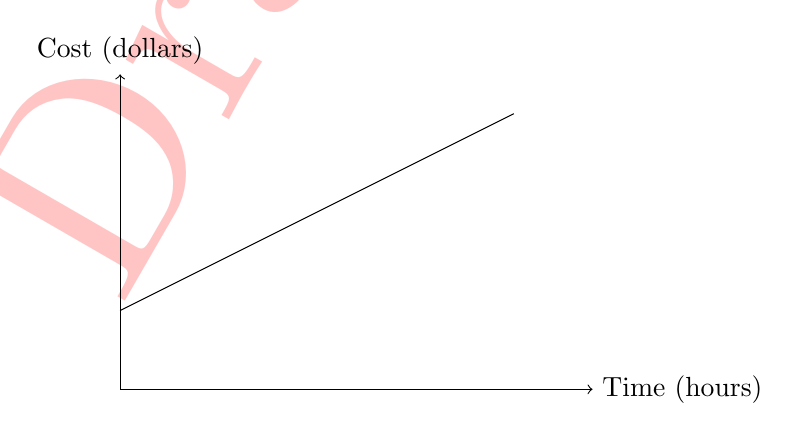
\begin{tikzpicture}
\draw[->] (0,0) -- (6,0) node[right] {Time (hours)};
\draw[->] (0,0) -- (0,4) node[above] {Cost (dollars)};
\draw (0,1) -- (5,3.5);
\end{tikzpicture}
\end{center}

\question For $2x + 3y = 12$, which equivalent form includes the $y$-intercept as a constant?
\begin{choices}
\choice $x = -\frac{3}{2}y + 6$
\choice $3y = -2x + 12$
\choice $\frac{2}{3}x - 4 + y = 0$
\choice $y = -\frac{2}{3}x + 4$
\end{choices}

\question Line $l$ passes through $(-2,3)$ and $(3,13)$. What is the $y$-intercept?

\question For $5x - 8y = 40$, $y$-intercept is $(0,c)$. What is c?

\question What is the $y$-coordinate of the $y$-intercept of $7x = 6 \left( 15 + \frac{9x}{4} - \frac{4y}{7} \right)$?

\question Linear function $f$ has negative slope and $y$-intercept $(0,k)$, $k > 0$. Which must be true?
\begin{choices}
\choice If $a > b$, then $f(a) < f(b)$
\choice If $a < 0$, then $f(a) > k$
\choice If $a > 0$, then $f(a) > 0$
\end{choices}
\begin{choices}
\choice I and II
\choice I and III
\choice II and III
\choice I, II, III
\end{choices}

\question Daily profit graph: Interpret $y$-intercept.
\begin{choices}
\choice Price per cake
\choice Cost per cake
\choice Daily running cost
\choice Cost of unsold cakes
\end{choices}

\question In $p = 900 - 10t$, interpret 900.
\begin{choices}
\choice Starting price
\choice Final price
\choice Price increase per second
\choice Auction time
\end{choices}

\question In $y = 1.30x - 1.50$, interpret 1.50.
\begin{choices}
\choice Bank fee in euros
\choice Bank fee in dollars
\choice USD to euro rate
\choice Euro to USD rate
\end{choices}

\question The relationship between the daily profit y, in dollars, of a bakery and the number of cakes sold by the bakery is graphed in the xy-plane below:
\begin{center}
\includegraphics[width=0.5\linewidth]{Screenshot 2025-06-24 at 19.14.03.png}
\end{center}

\question What does the slope represent?
\begin{choices}
\choice Price per cake
\choice Profit per cake
\choice Total profit
\choice Cakes for $100 profit
\end{choices}

\question Interpret $y$-intercept.
\begin{choices}
\choice Price per cake
\choice Cost per cake
\choice Daily running cost
\choice Cost of unsold cakes
\end{choices}

\question For $x + 2y = 1$, which form has the $y$-intercept as a constant or coefficient?
\begin{choices}
\choice $x + 2y - 1 = 0$
\choice $y = \frac{1}{2} - \frac{1}{2}x$
\choice $2y = 1 - x$
\choice $x = 1 - 2y$
\end{choices}

\question What is the $y$-intercept of $y = 4x - 1$?

\question Which equation matches the graph?
\begin{center}
\begin{tikzpicture}
\draw[->] (-2,0) -- (2,0) node[right] {$x$};
\draw[->] (0,-1) -- (0,3) node[above] {$y$};
\draw[domain=-1.5:0.5] plot (\x, {3*\x + 1});
\end{tikzpicture}
\end{center}
\begin{choices}
\choice $y = \frac{1}{3}x + 1$
\choice $y = x + 1$
\choice $y = x + 3$
\choice $y = 3x + 1$
\end{choices}

\question Which equation has slope 4 and passes through $(0,-3)$?
\begin{choices}
\choice $y = -4x + 3$
\choice $y = -3x + 4$
\choice $y = 4x - 3$
\choice $y = 3x - 4$
\end{choices}

\question About $2y - 3x = -4$, which is true?
\begin{choices}
\choice Negative slope, positive $y$-intercept
\choice Negative slope, negative $y$-intercept
\choice Positive slope, positive $y$-intercept
\choice Positive slope, negative $y$-intercept
\end{choices}

\question Line has slope 2 and passes through $(0,7)$. What is $f(2)$?
\begin{choices}
\choice 9
\choice 11
\choice 14
\choice 16
\end{choices}

\question Cereal: 28 oz initially, 2.4 oz eaten/day. Which represents remaining $C$ after $d$ days?
\begin{choices}
\choice $C = -2.4d + 28$
\choice $C = -2.4d - 28$
\choice $C = 2.4d + 28$
\choice $C = 2.4d - 28$
\end{choices}

\question College charges $900/credit + $1000/month room/board. For $x$ credits in 4 months, total charge $y$?
\begin{choices}
\choice $y = 900x + 4000$
\choice $y = 1000x + 3600$
\choice $y = 3600x + 4000$
\choice $y = \frac{900}{x} + 4000$
\end{choices}

\question Linear relationship:
\begin{center}
\begin{tabular}{|c|c|}
\hline
$s$ & $t$ \\
\hline
-5 & 0 \\
0 & 5 \\
\hline
\end{tabular}
\end{center}
Which equation?
\begin{choices}
\choice $t = -s - 5$
\choice $t = -s + 5$
\choice $t = s - 5$
\choice $t = s + 5$
\end{choices}

\question Which equation matches the graph?
\begin{center}
\includegraphics[width=0.5\linewidth]{Screenshot 2025-06-24 at 19.04.45.png}
\end{center}
\begin{choices}
\choice $y = -\frac{1}{2}x + 10$
\choice $y = -\frac{1}{2}x + 5$
\choice $y = -2x + 10$
\choice $y = -2x + 5$
\end{choices}

\question Equation with slope 2 through $(0,-3)$?
\begin{choices}
\choice $y = -3x + 2$
\choice $y = -3x - 2$
\choice $y = 2x + 3$
\choice $y = 2x - 3$
\end{choices}

\question $s(p) = 16,000 - 4.5p$ gives free space with $p$ photos (4.5 MB each). If 1500 photos, free space?

\question Carol buys 45 figures: first 30 at $d+5$ each, excess at $d$ each. Total cost $A$?
\begin{choices}
\choice $A = 30d + 45$
\choice $A = 30d + 150$
\choice $A = 45d + 45$
\choice $A = 45d + 150$
\end{choices}

\question Line $y = mx + b$ passes through $(-20,0)$ and $(0,40)$. What is $m$?

\question $f(x) = px + 8$ has $x$-intercept 4. What is $p$?
\begin{choices}
\choice -2
\choice 1
\choice $\frac{1}{2}$
\choice 2
\end{choices}

\question Equation $2,000 - 61k = 48$ models bird population $k$ years after 1962. Interpret 61.
\begin{choices}
\choice Population after $k$ years
\choice $k$ when population=48
\choice Difference 1962 and $k$ years
\choice Average decrease per year
\end{choices}

\question Linear function $f$:
\begin{center}
\begin{tabular}{|c|c|}
\hline
$x$ & $f(x)$ \\
\hline
8 & 12 \\
12 & 17 \\
\hline
\end{tabular}
\end{center}
$f(x) = ax + b$. What is $a + b$?

\question Values for $h$:
\begin{center}
\begin{tabular}{|c|c|}
\hline
$x$ & $h(x)$ \\
\hline
-7 & -11 \\
2 & 7 \\
4 & 11 \\
\hline
\end{tabular}
\end{center}
What is $h(8)$?
\begin{choices}
\choice 15
\choice 19
\choice 21
\choice 22
\end{choices}

\question Consultant charges $408 first hour + $204/additional hour. Charge for $h$ hours?
\begin{choices}
\choice $C(h) = 204h + 204$
\choice $C(h) = 204h + 408$
\choice $C(h) = 408h + 204$
\choice $C(h) = 408h + 612$
\end{choices}

\question In $17h + 45 = 164$, interpret 164.
\begin{choices}
\choice One-time fee
\choice Hours worked
\choice Charge per hour
\choice Total charge
\end{choices}

\question $p = 873 - 88t$ models pressure after $t$ hours. Pressure after 1 hour?
\begin{choices}
\choice 829
\choice 785
\choice 741
\choice 697
\end{choices}

\question Line through $(5,7)$ and $(3,11)$. Which equation?
\begin{choices}
\choice $f(x) = \frac{1}{2}x + \frac{9}{2}$
\choice $f(x) = -\frac{1}{2}x + \frac{19}{2}$
\choice $f(x) = 2x - 3$
\choice $f(x) = -2x + 17$
\end{choices}

\question Graph of $15x + By = 60$. What is $B$?
\begin{choices}
\choice $\frac{3}{4}$
\choice 3
\choice 4
\choice 20
\end{choices}

\question $w(t) = 3.1t - 1.7$ models pig weight at $t$ months. Interpret $w(7) = 20$.
\begin{choices}
\choice 20 pounds at 7 months
\choice 7 pounds at 20 months
\choice 20 pound increase in month 7
\choice 7 pound increase in month 20
\end{choices}

\question Line through $(0,2)$ and $(8,0)$ is $ax + by = 1$. What is $a$?

\question Consultant charges $444 first hour + $222/additional hour. Charge for $h$ hours?
\begin{choices}
\choice $C(h) = 222h + 222$
\choice $C(h) = 222h + 444$
\choice $C(h) = 444h + 222$
\choice $C(h) = 444h + 666$
\end{choices}

\question Linear model: 59k in 1991, 222k in 2011, $x$k in 2015. What is $x$?

\question Equipment rental: $350 first day + $175/additional day. Cost for $x$ days ($x \leq 5$)?
\begin{choices}
\choice $y = 175x + 175$
\choice $y = 350x - 175$
\choice $y = 175x + 350$
\choice $y = 350x + 175$
\end{choices}

\question $f(t) = 50 + 55t$ models bank account after $t$ deposits. Interpret 55.
\begin{choices}
\choice Increase of $55 per deposit
\choice Total 55 deposits
\choice Initial $55
\choice $55 after 1 deposit
\end{choices}

\question Bus rental: $750 first 2 hours + $50/additional hour. Total cost $1050 for $t$ hours ($t > 2$). Equation?
\begin{choices}
\choice $750(t - 2) + 50t = 1050$
\choice $750(2t) + 50t = 1050$
\choice $750 + 50(t - 2) = 1050$
\choice $750 + 50(2t) = 1050$
\end{choices}

\question Bear weight: 389 lb initially, loses 0.9 lb/day. Days to weigh 380 lb?

\question Linear profit: $320 at 6 items, $640 at 10 items. Equation?
\begin{choices}
\choice $f(x) = 180x - 640$
\choice $f(x) = 64x$
\choice $f(x) = 80x - 10$
\choice $f(x) = 80x - 160$
\end{choices}

\question Savings: Start $700, deposit $45/week. Amount after 6 weeks?
\begin{choices}
\choice 430
\choice 745
\choice 751
\choice 970
\end{choices}

\question Equipment rental: $64n first day + $32n/additional day. Cost for $x$ days?
\begin{choices}
\choice $C(x) = 32nx + 32n$
\choice $C(x) = 32nx + 64n$
\choice $C(x) = 64nx + 32n$
\choice $C(x) = 64nx - 32n$
\end{choices}

\question Colony: $y = 0.67x + 2.6$ predicts larvae from $x$ worker ants. If $x = 46$, predicted larvae?
\begin{choices}
\choice 33
\choice 49
\choice 65
\choice 150
\end{choices}

\question $P_1 = 10h + 101$, $P_2 = 10d + 311$. Interpret 311.
\begin{choices}
\choice Total pressure at depth $d$
\choice Pressure increase per meter
\choice Pressure increase for $d$ meters
\choice Total pressure at start of descent
\end{choices}

\question Train cars vs passengers:
\begin{center}
\begin{tabular}{|c|c|}
\hline
Cars & Passengers \\
\hline
4 & 164 \\
6 & 242 \\
8 & 320 \\
\hline
\end{tabular}
\end{center}
Which equation?
\begin{choices}
\choice $39c - p = -8$
\choice $39c - p = 8$
\choice $39p - c = -8$
\choice $39p - c = 8$
\end{choices}

\question $17.5x + 28.75y = 530$. How much more per ton of rock than per cubic yard of mulch?

\question Photosynthetic rate $P(x)$ increases 0.43 when energy increases 5. $P(300) = 9.8$. Equation?
\begin{choices}
\choice $P(x) = 0.026x + 9.8$
\choice $P(x) = 0.026x + 2$
\choice $P(x) = 9.8x + 0.026$
\choice $P(x) = 9.8x - 2,930.2$
\end{choices}

\question Star cluster mass 132.77 quettagrams. Graph models combinations of $x$ M-type and $y$ K-type stars. Estimated mass per star?
\begin{choices}
\choice 828
\choice 973
\choice 52,992
\choice 79,786
\end{choices}

\question Adriana's travel time:
\begin{center}
\begin{tabular}{|c|c|}
\hline
Distance (miles) & Time (minutes) \\
\hline
0.06 & 3 \\
0.28 & 14 \\
0.34 & 17 \\
\hline
\end{tabular}
\end{center}
Which equation?
\begin{choices}
\choice $t = \frac{1}{50}d$
\choice $t = \frac{1}{2}d$
\choice $t = 2d$
\choice $t = 50d$
\end{choices}

\question $T(x) = 61 - 8x$ estimates temperature $x$ hours after 10 a.m. Interpret $T(5) = 21$.
\begin{choices}
\choice 21°F at 5 hours after 10 a.m.
\choice 21°F decrease 5 hours before 10 a.m.
\choice 21°F decrease at 5 hours after 10 a.m.
\choice 21°F at 5 hours before 10 a.m.
\end{choices}

\question Linear relationship:
\begin{center}
\begin{tabular}{|c|c|}
\hline
$x$ & $y$ \\
\hline
$-2s$ & 20 \\
$-s$ & 16 \\
$s$ & 8 \\
\hline
\end{tabular}
\end{center}
Which equation?
\begin{choices}
\choice $sx + 4y = 12s$
\choice $4x + sy = 12s$
\choice $4x + sy = 12$
\choice $sx + 4y = 12$
\end{choices}

\question Computer repair: $160 first 2 hours + hourly fee. Total for 4 hours is $240. Cost for $x$ hours ($x \geq 2$)?
\begin{choices}
\choice $f(x) = 40x + 80$
\choice $f(x) = 40x + 160$
\choice $f(x) = 60x$
\choice $f(x) = 60x + 160$
\end{choices}

\question $y$ is 49 more than twice $x$. Equation?
\begin{choices}
\choice $y = 2x + 49$
\choice $y = 49x + 2$
\choice $y = 51x - 2$
\choice $y = 51x + 49$
\end{choices}

\question The graph of line $g$ is shown in the $xy$-plane. Line $k$ is defined by the equation
\[
165x + py = w,
\]
where $p$ and $w$ are constants. If line $k$ is graphed in this $xy$-plane resulting in a system of two linear equations with infinitely many solutions, what is the value of $p + w$?

\begin{center}
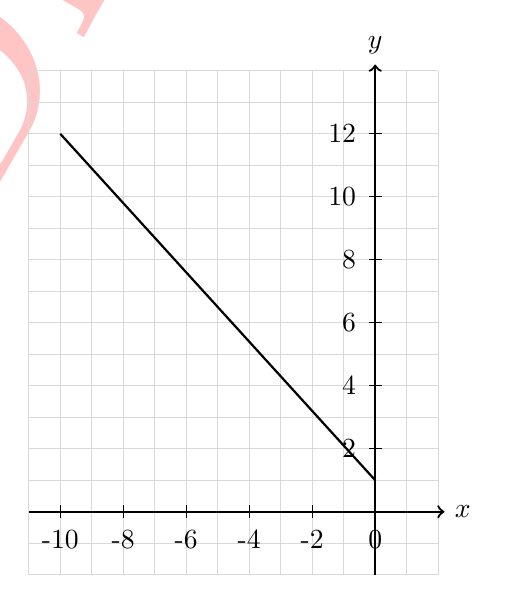
\begin{tikzpicture}[scale=0.4]

% Draw grid
\draw[step=1cm, color=gray!30, thin] (-11,-2) grid (2,14);

% Axes
\draw[->, thick] (-11,0) -- (2.2,0) node[right] {$x$};
\draw[->, thick] (0,-2) -- (0,14.2) node[above] {$y$};

% Axis ticks every 2 units
\foreach \x in {-10,-8,...,0} {
    \draw (\x,0.2) -- (\x,-0.2);
    \node[below] at (\x,-0.3) {\x};
}
\foreach \y in {2,4,...,12} {
    \draw (0.2,\y) -- (-0.2,\y);
    \node[left] at (-0.3,\y) {\y};
}

% Line g through (-10,12) and (0,1)
\draw[thick, domain=-10:0] plot (\x, {-11/10*\x + 1});

\end{tikzpicture}
\end{center}

\question For $7x - 4y = -84$, which table?
\begin{choices}
\choice 
    \begin{tabular}{|c|c|c|c|}
    \hline
    $x$ & 0 & 4 & 8 \\
    $y$ & 21 & 28 & 35 \\
    \hline
    \end{tabular}
\choice 
    \begin{tabular}{|c|c|c|c|}
    \hline
    $x$ & 0 & 4 & 8 \\
    $y$ & 35 & 28 & 21 \\
    \hline
    \end{tabular}
\choice 
    \begin{tabular}{|c|c|c|c|}
    \hline
    $x$ & 21 & 28 & 35 \\
    $y$ & 0 & 4 & 8 \\
    \hline
    \end{tabular}
\choice 
    \begin{tabular}{|c|c|c|c|}
    \hline
    $x$ & 21 & 28 & 35 \\
    $y$ & 8 & 4 & 0 \\
    \hline
    \end{tabular}
\end{choices}

\question A certain open star cluster contains M-type stars and K-type stars. The estimated total mass of M-type and K-type stars in this open star cluster is 129{,}492 quettagrams. The graph shown models the possible combinations of the number of M-type stars, $x$, and K-type stars, $y$, that could be in this open star cluster if all the M-type stars have the same estimated mass and all the K-type stars have the same estimated mass. Based on the graph, which of the following is closest to the estimated mass, in quettagrams, of each M-type star in this cluster?

\begin{choices}
\choice 830
\choice 959
\choice 55{,}622
\choice 73{,}870
\end{choices}

\begin{center}
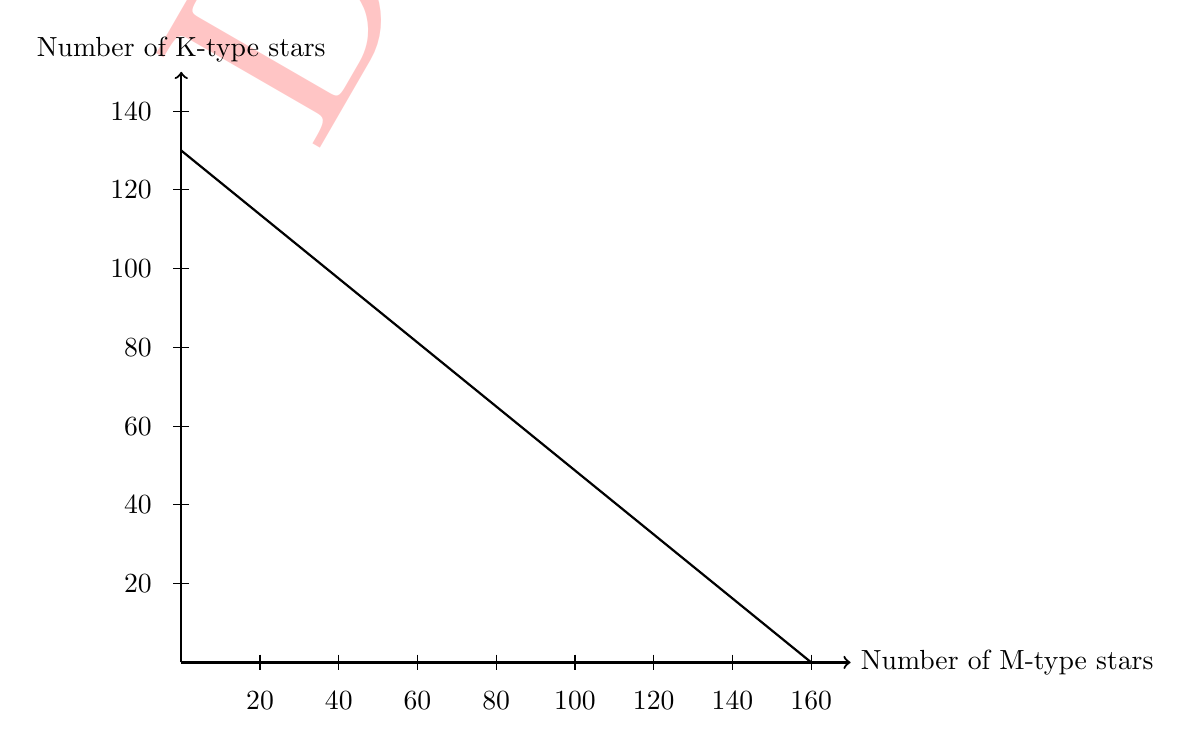
\begin{tikzpicture}[scale=0.05]

% Axes
\draw[->, thick] (0,0) -- (170,0) node[right] {Number of M-type stars};
\draw[->, thick] (0,0) -- (0,150) node[above] {Number of K-type stars};

% Axis ticks and labels
\foreach \x in {20,40,...,160} {
    \draw (\x,2) -- (\x,-2);
    \node[below] at (\x,-5) {\x};
}

\foreach \y in {20,40,...,140} {
    \draw (2,\y) -- (-2,\y);
    \node[left] at (-5,\y) {\y};
}

% Line (approximate): from (0,130) to (160,0)
\draw[thick] (0,130) -- (160,0);

\end{tikzpicture}
\end{center}

\question $f(x) = 39 - 0.18x$ models water height. Interpret 39.
\begin{choices}
\choice Initial height
\choice Final height
\choice Change per day
\choice Days to evaporate
\end{choices}

\question System: $y = \frac{2}{7}x + 3$ has infinitely many solutions. If second equation $y = mx + b$, what is $b$?
\begin{choices}
\choice -3
\choice $-\frac{1}{3}$
\choice $\frac{1}{3}$
\choice 3
\end{choices}

\question Equipment rental: $270 first day + $135/additional day. Cost for $x$ days ($x \leq 5$)?
\begin{choices}
\choice $y = 135x + 135$
\choice $y = 270x - 135$
\choice $y = 270x + 135$
\choice $y = 135x + 270$
\end{choices}

\question Roof area vs water drained:
\begin{center}
\begin{tabular}{|c|c|}
\hline
Area (sq ft) & Water (gallons) \\
\hline
2,520 & 4,536 \\
3,780 & 6,804 \\
5,040 & 9,072 \\
\hline
\end{tabular}
\end{center}
Which equation?
\begin{choices}
\choice $f(x) = 0.6x$
\choice $f(x) = 1.8x$
\choice $f(x) = 2,268.0x$
\choice $f(x) = \frac{x}{6}$
\end{choices}

\question Museum: $22/person first 25 + $14/additional. Charge for $n$ people ($n \geq 25$)?
\begin{choices}
\choice $f(n) = 14n + 200$
\choice $f(n) = 14n + 22$
\choice $f(n) = 14n + 550$
\choice $f(n) = 36n - 350$
\end{choices}

\question The graph of line $g$ is shown in the $xy$-plane. Line $k$ is defined by the equation
\[
165x + py = w,
\]
where $p$ and $w$ are constants. If line $k$ is graphed in this $xy$-plane resulting in a system of two linear equations with infinitely many solutions, what is the value of $p + w$?

\begin{center}
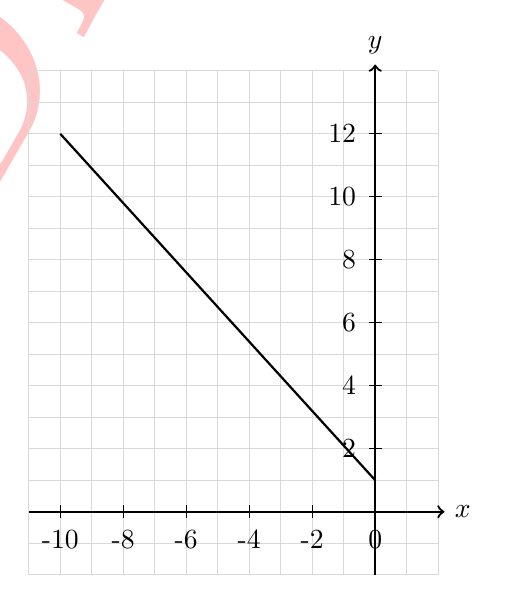
\begin{tikzpicture}[scale=0.4]

% Draw grid
\draw[step=1cm, color=gray!30, thin] (-11,-2) grid (2,14);

% Axes
\draw[->, thick] (-11,0) -- (2.2,0) node[right] {$x$};
\draw[->, thick] (0,-2) -- (0,14.2) node[above] {$y$};

% Axis ticks every 2 units
\foreach \x in {-10,-8,...,0} {
    \draw (\x,0.2) -- (\x,-0.2);
    \node[below] at (\x,-0.3) {\x};
}
\foreach \y in {2,4,...,12} {
    \draw (0.2,\y) -- (-0.2,\y);
    \node[left] at (-0.3,\y) {\y};
}

% Line g through (-10,12) and (0,1)
\draw[thick, domain=-10:0] plot (\x, {-11/10*\x + 1});

\end{tikzpicture}
\end{center}

\question A bank account was opened with an initial deposit. Over the next several months, regular deposits were made into this account and there were no withdrawals made during this time. The graph of the function y = f(x) estimates the account balance, in dollars, in this bank account x months since the initial deposit. To the nearest whole dollar, what is the amount of the initial deposit estimated by the graph?
\begin{center}
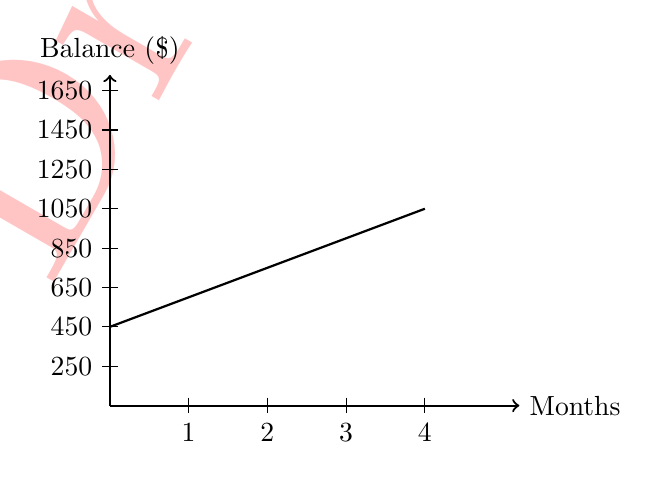
\begin{tikzpicture}[scale=1]
% Axes
\draw[->, thick] (0,0) -- (5.2,0) node[right] {Months};
\draw[->, thick] (0,0) -- (0,4.2) node[above] {Balance (\$)};

% Ticks on x-axis (Months)
\foreach \x/\xtext in {1/1, 2/2, 3/3, 4/4} {
    \draw (\x,0.1) -- (\x,-0.1);
    \node[below] at (\x,-0.1) {\xtext};
}

% Ticks on y-axis (Balance)
\foreach \y/\ytext in {0.5/250, 1/450, 1.5/650, 2/850, 2.5/1050, 3/1250, 3.5/1450, 4/1650} {
    \draw (0.1,\y) -- (-0.1,\y);
    \node[left] at (-0.1,\y) {\ytext};
}

% Line from initial deposit
\draw[thick] (0,1) -- (4,2.5); % scaled: 1 = $450, 2.5 = $1050
\end{tikzpicture}
\end{center}

\question $F(m) = 7m$ models force. Interpret $F(4) = 28$.
\begin{choices}
\choice 28 newtons for 4 kg
\choice 4 newtons for 28 kg
\choice 4 newtons for 7 kg
\choice 28 newtons for 7 kg
\end{choices}

\question $13x + 14y = 423$ models shirt sales. Interpret $y$.
\begin{choices}
\choice Number of long-sleeved shirts
\choice Number of short-sleeved shirts
\choice Price of long-sleeved shirt
\choice Price of short-sleeved shirt
\end{choices}

\question $f(x) = -40x + 280$ models airplane height. Height at 4 minutes?
\begin{choices}
\choice 120
\choice 160
\choice 240
\choice 440
\end{choices}

\question Train cars vs passengers:
\begin{center}
\begin{tabular}{|c|c|}
\hline
Cars & Passengers \\
\hline
3 & 99 \\
5 & 161 \\
10 & 316 \\
\hline
\end{tabular}
\end{center}
Which equation?
\begin{choices}
\choice $31c - p = -6$
\choice $31c - p = 6$
\choice $31p - c = -6$
\choice $31p - c = 6$
\end{choices}

\question Linear relationship:
\begin{center}
\begin{tabular}{|c|c|}
\hline
$x$ & $y$ \\
\hline
-2 & 19 \\
0 & 31 \\
2 & 43 \\
\hline
\end{tabular}
\end{center}
If $Ax + By = C$, what is $\frac{A}{B}$?

\question Rectangular garden: length $x$, width $y$, fencing total 44 feet. Equation?
\begin{choices}
\choice $2x + 2y = 44$
\choice $x + y = 44$
\choice $2xy = 44$
\choice $xy = 44$
\end{choices}

\question Linear profit: $190 at 4 items, $670 at 10 items. Equation?
\begin{choices}
\choice $f(x) = 180x - 670$
\choice $f(x) = 67x$
\choice $f(x) = 80x - 10x$
\choice $f(x) = 80x - 130$
\end{choices}

\question Linear relationship:
\begin{center}
\begin{tabular}{|c|c|}
\hline
$x$ & $y$ \\
\hline
0 & 22 \\
1 & 23 \\
2 & 24 \\
\hline
\end{tabular}
\end{center}
Which equation?
\begin{choices}
\choice $y = x + 22$
\choice $y = 24x$
\choice $y = 24x + 2$
\choice $y = 22x$
\end{choices}

\question Container: 24 mL initially. Faucet adds 0.03 mL every 3 seconds. Volume $v$ after $t$ seconds (multiple of 3)?
\begin{choices}
\choice $v = 0.01t + 24$
\choice $v = 0.03t + 24$
\choice $v = 0.09t + 24$
\choice $v = 3t$
\end{choices}

\question Jenny made $x$ cookies/hour for 2 hours, Cara $y$ cookies/hour for 3 hours. Total cookies?
\begin{choices}
\choice $6xy$
\choice $3x + 2y$
\choice $2x + 3y$
\choice $5xy$
\end{choices}

\question $W = 42 - 7d$ models wills left. Interpret 42.
\begin{choices}
\choice Finish in 42 days
\choice 42 wills/day
\choice 6 wills/hour
\choice Start with 42 wills
\end{choices}

\question Skateboard: 8 ft/s at hilltop, 43 ft/s after 3.5 seconds. Acceleration (ft/s²)?
\begin{choices}
\choice 8
\choice 10
\choice 12
\choice 14
\end{choices}

\question Softball team: $75/member + $50 fee. Max members for $780?

\question $2.25x + 0.75y = 35$ for avocados and bananas. Interpret 35.
\begin{choices}
\choice Avocados/week
\choice Money spent/week
\choice Total fruits/week
\choice Difference avocados-bananas
\end{choices}

\question 5 burgers with tax: $30.97 (tax $0.22). Cost of 4 burgers without tax?
\begin{choices}
\choice 18.00
\choice 20.25
\choice 24.60
\choice 28.00
\end{choices}

\question $34c + 52t = 1070$ for trucks and cars. If 16 trucks, how many cars?

\question John's meal $y$, Matt's $y+6$. Split evenly. Each pays?
\begin{choices}
\choice $y$
\choice $y + 6$
\choice $y + 3$
\choice $2y + 6$
\end{choices}

\question James 40 shares, Danny 35, John 28. Share value $7. Total value?
\begin{choices}
\choice 441
\choice 476
\choice 721
\choice 796
\end{choices}

\question Cupcake company: 146/day in 2020, 12 less than half of last year. Last year average?

\question Jamie: pies 20 min, cookies 30 min/tray. Spends 8 hours, twice as many cookie trays as pies. How many cookie trays?
\begin{choices}
\choice 6
\choice 8
\choice 10
\choice 12
\end{choices}

\question Farmer: horses $1800, cows $1100. Budget $17,000, at least 13 animals. Max horses?

\question Two positive integers: product 84, smaller = $\frac{1}{2}$ larger + 1. Smaller?
\begin{choices}
\choice 5
\choice 6
\choice 7
\choice 12
\end{choices}

\question Dynamite: Monday 63 more than Tuesday. Total 873 sticks. Tuesday?
\begin{choices}
\choice 400
\choice 405
\choice 468
\choice 810
\end{choices}

\question Danny: $8.50/hour first 40 hours, 1.5 times after. Earned $505.75 last week. Total hours?

\question Train model: scale 1 cm : 5 m. Length 7.6 cm. New scale 1 cm : 10 m. New length?
\begin{choices}
\choice 10 cm longer
\choice 10 cm shorter
\choice Half as long
\choice Twice as long
\end{choices}

\question Woody: 13-19 logs/day, Willy: 7-16 logs/day. Days to chuck 175 logs?

\question Birthday party: $18,000. Initially $n$ family members split equally. After 3 refuse, each pays $1000 more. What is $n$?

\question Julie worked 3 less than twice Bruce's hours. Julie $J$ based on Bruce $B$?
\begin{choices}
\choice $J = 2B - 3$
\choice $J = 2 - 3B$
\choice $J = 2B + 3$
\choice $J = 3 - 2B$
\choice $J = -2B - 3$
\end{choices}

\question Line $r$ is defined by the equation $4x - 5y = 8$. Line $s$ is parallel to line $r$ in the $xy$-plane. What is the slope of line $s$?
\begin{choices}
\choice $\dfrac{5}{4}$
\choice $\dfrac{4}{5}$
\choice $-4$
\choice $-5$
\end{choices}

\question In the $xy$-plane, line $l$ passes through $(0,0)$ and is parallel to $y = 6x + 3$. If line $l$ also passes through $(3,d)$, what is $d$?

\question Line $r$ is defined by $4x - 7y = 3$. Line $s$ is parallel to line $r$. What is the slope of line $s$?
\begin{choices}
\choice $\dfrac{7}{4}$
\choice $\dfrac{4}{7}$
\choice $-4$
\choice $-7$
\end{choices}

\question Line $k$ is defined by $y = 6x + 5$. Line $j$ is parallel to line $k$ and passes through $(0,11)$. Which equation defines line $j$?
\begin{choices}
\choice $y = 6x + 11$
\choice $y = 11x + 5$
\choice $y = -6x + 11$
\choice $y = -11x + 5$
\end{choices}

\question Line $k$ is defined by $y = 4x + 1$. Line $j$ is parallel to line $k$ and passes through $(0,5)$. Which equation defines line $j$?
\begin{choices}
\choice $y = -5x + 1$
\choice $y = 5x + 1$
\choice $y = -4x + 5$
\choice $y = 4x + 5$
\end{choices}

\question Line $s$ passes through $(0,0)$ and is parallel to $y = 25x + 5$. If line $s$ also passes through $(2,d)$, what is $d$?
\begin{choices}
\choice 5
\choice 25
\choice 50
\choice 55
\end{choices}

\question Line $r$ is defined by $4x - 3y = 8$. Line $s$ is parallel to line $r$. What is the slope of line $s$?
\begin{choices}
\choice $-4$
\choice $-3$
\choice $\dfrac{3}{4}$
\choice $\dfrac{4}{3}$
\end{choices}

\question Line $p$ is defined by $y = 6x - 8$. Line $s$ is parallel to line $p$. What is the slope of line $s$?

\question Line $k$ is defined by $y = 7x + 2$. Line $j$ is parallel to line $k$ and passes through $(0,3)$. Which equation defines line $j$?
\begin{choices}
\choice $y = 7x + 3$
\choice $y = -3x + 3$
\choice $y = -7x + 3$
\choice $y = 3x + 3$
\end{choices}

\question Line $k$ is defined by $y = 6x + \dfrac{1}{9}$. Line $j$ is perpendicular to line $k$. What is the slope of line $j$?
\begin{choices}
\choice $-9$
\choice $-\dfrac{1}{6}$
\choice $\dfrac{1}{9}$
\choice $6$
\end{choices}

\question Line $k$ is shown in the $xy$-plane. Line $j$ (not shown) is perpendicular to line $k$ and passes through $(-12,-19)$. Which equation defines line $j$?
\begin{center}
\includegraphics[width=0.5\linewidth]{Screenshot 2025-06-24 at 16.45.48.png}
\end{center}
\begin{choices}
\choice $y = \dfrac{2}{3}x - 11$
\choice $y = \dfrac{2}{3}x - 27$
\choice $y = \dfrac{3}{2}x - 11$
\choice $y = \dfrac{3}{2}x - 27$
\end{choices}

\question Line $j$ is perpendicular to line $k$. What is the slope of line $j$?
\begin{center}
\includegraphics[width=0.5\linewidth]{Screenshot 2025-06-24 at 16.48.12.png}
\end{center}
\begin{choices}
\choice $-\dfrac{6}{5}$
\choice $\dfrac{6}{5}$
\choice $6$
\choice $-5$
\end{choices}

\question Lines $p$ and $q$ are perpendicular with $y$-intercept $-4$. Line $p$ crosses the $x$-axis at $x=3$. At which $x$ does line $q$ cross the $x$-axis?
\begin{choices}
\choice $\dfrac{4}{3}$
\choice $-4$
\choice $-\dfrac{3}{4}$
\choice $-\dfrac{16}{3}$
\choice $\dfrac{16}{3}$
\end{choices}

\question Line $k$ passes through $(2,4)$ and is perpendicular to $y = \dfrac{2}{3}x - 6$. Which is the equation for line $k$?
\begin{choices}
\choice $y = \dfrac{3}{2}x - 6$
\choice $y = -\dfrac{3}{2}x + 7$
\choice $y = \dfrac{2}{3}x + 7$
\choice $y = -\dfrac{2}{3}x + 7$
\choice $y = -\dfrac{3}{2}x - 6$
\end{choices}

\question Points $(4,10)$ and $(1,31)$ are on line $q$. Line $p$ is perpendicular to line $q$. Which equation could be for line $p$?
\begin{choices}
\choice $y = 7x + 28$
\choice $y = \dfrac{1}{7}x - \dfrac{5}{2}$
\choice $y = -7x + 10$
\choice $y = -\dfrac{1}{7}x + 2$
\end{choices}

\question Line $d$ is parallel to line $f$ with equation $y = \dfrac{3}{5}x + \dfrac{9}{2}$. Which could be the equation of line $d$?
\begin{choices}
\choice $3x + 5y = 20$
\choice $10x - 6y = 3$
\choice $9x - 15y = 40$
\choice $-5x + 3y = 18$
\end{choices}

\question Which equation could be for parallel line $b$?
\begin{center}
\includegraphics[width=0.5\linewidth]{Screenshot 2025-06-24 at 16.50.18.png}
\end{center}
\begin{choices}
\choice $y = x - 3$
\choice $y = \dfrac{1}{2}x - 2$
\choice $y = 2x + 4$
\choice $y = -2x - 5$
\end{choices}

\question Lines $l$ and $k$ are parallel. Equation for $l$ is $x + 4y = -5$, line $k$ passes through $(2,8)$. What is the $x$-intercept for line $k$?

\question Lines $l$ and $k$ are parallel. Line $l$ passes through $(-1,-7)$ and $(1,3)$. If $(a,b)$ is on line $k$, which is another point on line $k$?
\begin{choices}
\choice $(a-1,b-5)$
\choice $(a-1,b+5)$
\choice $(a+5,b+1)$
\choice $(a+5,b-1)$
\end{choices}

\question The graphs of $7x + 11y = 100$ and $ax + by = 10b$ are perpendicular. Which pair represents parallel lines?
\begin{choices}
\choice $7x - 11y = 10$, $ax + by = 10b$
\choice $7x + 33y = 100$, $2ax - 3by = 50b$
\choice $33x - 7y = 100$, $3ax + by = b$
\choice $11x + 7y = 100$, $ax + by = 10b$
\end{choices}

\question What is the slope of a line perpendicular to $6x = 4y + 10$?

\question Line $k$ is defined by $3x + 5y = 24$. Line $a$ is perpendicular to line $k$. What is the slope of line $a$?

\question $g(x)$ is perpendicular to $f(x)$. Which could define $g(x)$?
\begin{center}
\includegraphics[width=0.5\linewidth]{Screenshot 2025-06-24 at 16.51.36.png}
\end{center}
\begin{choices}
\choice $g(x) = -2x - 2$
\choice $g(x) = -\dfrac{1}{2}x + 4$
\choice $g(x) = \dfrac{1}{2}x + 2$
\choice $g(x) = 2x - 3$
\end{choices}

\question Line $m$ is defined by $y = -\dfrac{3}{5}x + 7$. Line $k$ is perpendicular to $m$ and passes through $(6,13)$. Which equation defines $k$?
\begin{choices}
\choice $y = \dfrac{5}{3}x + \dfrac{1}{7}$
\choice $y = \dfrac{5}{3}x + 3$
\choice $y = \dfrac{5}{3}x + 7$
\choice $y = \dfrac{5}{3}x + \dfrac{47}{3}$
\end{choices}

\question Lines $t$ and $v$ are perpendicular. Equation of $t$ is $4x + 3y = 10$, line $v$ passes through $(-3,3)$. What is the $y$-intercept of line $v$?

\question Which equation's graph is perpendicular to $4x - 3y = 10$?
\begin{choices}
\choice $-4y + 3x = 3$
\choice $6x + 8y = -7$
\choice $2x - 3y = 10$
\choice $-4x + 3y = 10$
\end{choices}

\question Line $l$ passes through $(2,6)$ and is perpendicular to $2x + 3y = 6$. If $l$ crosses the $y$-axis at $(0,b)$, what is $b$?

\question Line $m$ is perpendicular to line $l$: $y = \dfrac{4}{3}x + 4$. Which is the equation of line $m$?
\begin{choices}
\choice $4x + 3y + 3 = 0$
\choice $4x - 3y + 3 = 0$
\choice $3x - 4y + 12 = 0$
\choice $3x + 4y + 12 = 0$
\end{choices}

\question The graphs of $3x + 8y = 10$ and $ax + by = 10$ are perpendicular. Which pair are also perpendicular?
\begin{choices}
\choice $12x + 11y = 40$, $2ax + by = 40$
\choice $6x - 16y = 10$, $ax - 3by = 40$
\choice $24x + 11y = 40$, $ax + 4by = 40$
\choice $6x + 22y = 40$, $-2ax + by = 40$
\end{choices}

\question What is the slope of a line perpendicular to $y = -\dfrac{1}{4}x + 5$?

\question Which equation is parallel to line $l$?
\begin{center}
\includegraphics[width=0.5\linewidth]{Screenshot 2025-06-24 at 16.53.00.png}
\end{center}
\begin{choices}
\choice $y = -\dfrac{2}{3}x + 2$
\choice $y = \dfrac{2}{3}x + 10$
\choice $y = \dfrac{3}{2}x - 4$
\choice $y = 3x - 1$
\end{choices}

\question Line $k$ passes through $(1,5)$ and is perpendicular to $y = \dfrac{1}{2}x + 3$. Which equation defines $k$?
\begin{choices}
\choice $y = -2x + 3$
\choice $y = -2x + 7$
\choice $y = -\dfrac{1}{2}x + \dfrac{11}{2}$
\choice $y = \dfrac{1}{2}x + \dfrac{9}{2}$
\end{choices}

\question Line $s$ is parallel to $r$ and passes through $(1,-1)$. Which point lies on $s$?
\begin{center}
\includegraphics[width=0.5\linewidth]{Screenshot 2025-06-24 at 16.55.07.png}
\end{center}
\begin{choices}
\choice $(-3,-3)$
\choice $(-2,-2)$
\choice $(0,-2)$
\choice $(4,0)$
\end{choices}

\question The linear function $f$ is perpendicular to $g$ (not shown). Their graphs intersect at $\left(1,\dfrac{5}{2}\right)$. What is $g(-1)$?

\question Line $j$ is defined by $4x + 20y = 5$. Line $k$ is parallel to $j$. What is the slope of $k$?
\begin{choices}
\choice $-5$
\choice $-\dfrac{1}{5}$
\choice $\dfrac{1}{5}$
\choice $5$
\end{choices}

\question Line $p$ passes through $(1,n)$. Line $q$ intersects $p$ at $(0,0)$ and is perpendicular to $p$. Which point must lie on $q$?
\begin{choices}
\choice $(-n,-1)$
\choice $(n,-1)$
\choice $(n,1)$
\choice $(1,-n)$
\end{choices}

\question $ax - by = 5$ is perpendicular to $11x - 4y = 5$. Which line is perpendicular to $11x + 12y = 5$?
\begin{choices}
\choice $ax - 3by = 5$
\choice $ax + 3by = 5$
\choice $3ax - by = 5$
\choice $3ax + by = 5$
\end{choices}

\question Which line passes through $(-4,1)$ and is parallel to $4x - 2y = 3$?
\begin{choices}
\choice $y = 2x - 9$
\choice $y = 2x + 9$
\choice $y = -2x - 9$
\choice $y = -2x + 9$
\end{choices}

\question Which line passes through $(-4,1)$ and is perpendicular to $4x - 2y = 3$?
\begin{choices}
\choice $y = -\dfrac{1}{2}x - 1$
\choice $y = -\dfrac{1}{2}x + 1$
\choice $y = \dfrac{1}{2}x - 1$
\choice $y = \dfrac{1}{2}x + 1$
\end{choices}

\question Which linear equation is for the line parallel to $3x + 4y = 12$ through $(-2,-3)$?
\begin{choices}
\choice $y - 3 = -\dfrac{3}{4}(x - 2)$
\choice $y + 3 = -\dfrac{4}{3}(x + 2)$
\choice $y - 3 = -\dfrac{4}{3}(x - 2)$
\choice $y + 3 = -\dfrac{3}{4}(x + 2)$
\end{choices}

\question The lines $6x + 11y = 40$ and $ax + by = 10b$ are perpendicular. Which pair represents parallel lines?
\begin{choices}
\choice $7x - 11y = 10$, $ax + by = 10b$
\choice $7x + 33y = 100$, $2ax - 3by = 50b$
\choice $33x - 7y = 100$, $3ax + by = b$
\choice $11x + 7y = 100$, $ax + by = 10b$
\end{choices}

\question What is the slope of a line perpendicular to $6x = 4y + 10$?

\question Line $k$ is defined by $3x + 5y = 24$. Line $a$ is perpendicular to line $k$. What is the slope of line $a$?

\question $g(x)$ is perpendicular to $f(x)$. Which could define $g(x)$?
\begin{center}
\includegraphics[width=0.5\linewidth]{Screenshot 2025-06-24 at 16.51.36.png}
\end{center}
\begin{choices}
\choice $g(x) = -2x - 2$
\choice $g(x) = -\dfrac{1}{2}x + 4$
\choice $g(x) = \dfrac{1}{2}x + 2$
\choice $g(x) = 2x - 3$
\end{choices}

\question Line $m$ is defined by $y = -\dfrac{3}{5}x + 7$. Line $k$ is perpendicular to $m$ and passes through $(6,13)$. Which equation defines $k$?
\begin{choices}
\choice $y = \dfrac{5}{3}x + \dfrac{1}{7}$
\choice $y = \dfrac{5}{3}x + 3$
\choice $y = \dfrac{5}{3}x + 7$
\choice $y = \dfrac{5}{3}x + \dfrac{47}{3}$
\end{choices}

\question Lines $t$ and $v$ are perpendicular. Equation of $t$ is $4x + 3y = 10$, line $v$ passes through $(-3,3)$. What is the $y$-intercept of line $v$?

\question Which equation's graph is perpendicular to $4x - 3y = 10$?
\begin{choices}
\choice $-4y + 3x = 3$
\choice $6x + 8y = -7$
\choice $2x - 3y = 10$
\choice $-4x + 3y = 10$
\end{choices}

\question Line $l$ passes through $(2,6)$ and is perpendicular to $2x + 3y = 6$. If $l$ crosses the $y$-axis at $(0,b)$, what is $b$?

\question Line $m$ is perpendicular to line $l$: $y = \dfrac{4}{3}x + 4$. Which is the equation of line $m$?
\begin{choices}
\choice $4x + 3y + 3 = 0$
\choice $4x - 3y + 3 = 0$
\choice $3x - 4y + 12 = 0$
\choice $3x + 4y + 12 = 0$
\end{choices}

\question The graphs of $3x + 8y = 10$ and $ax + by = 10$ are perpendicular. Which pair also represents perpendicular lines?
\begin{choices}
\choice $3x - 8y = 10$, $ax + by = 10$
\choice $6x - 16y = 10$, $2ax + 2by = 5$
\choice $3x + 16y = 10$, $2ax + by = 10$
\choice $3x + 16y = 10$, $ax + 2by = 10$
\end{choices}

\question What is the slope of a line perpendicular to $y = -\dfrac{1}{4}x + 5$?

\question Which equation is parallel to line $l$?
\begin{center}
\includegraphics[width=0.5\linewidth]{Screenshot 2025-06-24 at 16.53.00.png}
\end{center}
\begin{choices}
\choice $y = -\dfrac{2}{3}x + 2$
\choice $y = \dfrac{2}{3}x + 10$
\choice $y = \dfrac{3}{2}x - 4$
\choice $y = 3x - 1$
\end{choices}

\question Line $k$ passes through $(1,5)$ and is perpendicular to $y = \dfrac{1}{2}x + 3$. Which equation defines $k$?
\begin{choices}
\choice $y = -2x + 3$
\choice $y = -2x + 7$
\choice $y = -\dfrac{1}{2}x + \dfrac{11}{2}$
\choice $y = \dfrac{1}{2}x + \dfrac{9}{2}$
\end{choices}

\question Line $s$ is parallel to $r$ and passes through $(1,-1)$. Which point lies on $s$?
\begin{center}
\includegraphics[width=0.5\linewidth]{Screenshot 2025-06-24 at 16.55.07.png}
\end{center}
\begin{choices}
\choice $(-3,-3)$
\choice $(-2,-2)$
\choice $(0,-2)$
\choice $(4,0)$
\end{choices}

\question The linear function $f$ is perpendicular to $g$ (not shown). Their graphs intersect at $\left(1,\dfrac{5}{2}\right)$. What is $g(-1)$?

\question Line $j$ is defined by $4x + 20y = 5$. Line $k$ is parallel to $j$. What is the slope of $k$?
\begin{choices}
\choice $-5$
\choice $-\dfrac{1}{5}$
\choice $\dfrac{1}{5}$
\choice $5$
\end{choices}

\question Line $p$ passes through $(1,n)$. Line $q$ intersects $p$ at $(0,0)$ and is perpendicular to $p$. Which point must lie on $q$?
\begin{choices}
\choice $(-n,-1)$
\choice $(n,-1)$
\choice $(n,1)$
\choice $(1,-n)$
\end{choices}

\question $ax - by = 5$ is perpendicular to $11x - 4y = 5$. Which line is perpendicular to $11x + 12y = 5$?
\begin{choices}
\choice $ax - 3by = 5$
\choice $ax + 3by = 5$
\choice $3ax - by = 5$
\choice $3ax + by = 5$
\end{choices}

\question Which line passes through $(-4,1)$ and is parallel to $4x - 2y = 3$?
\begin{choices}
\choice $y = 2x - 9$
\choice $y = 2x + 9$
\choice $y = -2x - 9$
\choice $y = -2x + 9$
\end{choices}

\question Which line passes through $(-4,1)$ and is perpendicular to $4x - 2y = 3$?
\begin{choices}
\choice $y = -\dfrac{1}{2}x - 1$
\choice $y = -\dfrac{1}{2}x + 1$
\choice $y = \dfrac{1}{2}x - 1$
\choice $y = \dfrac{1}{2}x + 1$
\end{choices}

\question Which linear equation is for the line parallel to $3x + 4y = 12$ through $(-2,-3)$?
\begin{choices}
\choice $y - 3 = -\dfrac{3}{4}(x - 2)$
\choice $y + 3 = -\dfrac{4}{3}(x + 2)$
\choice $y - 3 = -\dfrac{4}{3}(x - 2)$
\choice $y + 3 = -\dfrac{3}{4}(x + 2)$
\end{choices}

\question The lines $6x + 11y = 40$ and $ax + by = 40$ are perpendicular. Which pair are also perpendicular?
\begin{choices}
\choice $12x + 11y = 40$, $2ax + by = 40$
\choice $6x + 33y = 40$, $ax - 3by = 40$
\choice $24x + 11y = 40$, $ax + 4by = 40$
\choice $6x + 22y = 40$, $-2ax + by = 40$
\end{choices}

\question What is the slope of a line perpendicular to $y = -\dfrac{1}{4}x + 5$?

\question Which equation is parallel to line $l$?
\begin{center}
\includegraphics[width=0.5\linewidth]{Screenshot 2025-06-24 at 16.53.00.png}
\end{center}
\begin{choices}
\choice $y = -\dfrac{2}{3}x + 2$
\choice $y = \dfrac{2}{3}x + 10$
\choice $y = \dfrac{3}{2}x - 4$
\choice $y = 3x - 1$
\end{choices}

\question Line $k$ passes through $(1,5)$ and is perpendicular to $y = \dfrac{1}{2}x + 3$. Which equation defines $k$?
\begin{choices}
\choice $y = -2x + 3$
\choice $y = -2x + 7$
\choice $y = -\dfrac{1}{2}x + \dfrac{11}{2}$
\choice $y = \dfrac{1}{2}x + \dfrac{9}{2}$
\end{choices}

\question Line $s$ is parallel to $r$ and passes through $(1,-1)$. Which point lies on $s$?
\begin{center}
\includegraphics[width=0.5\linewidth]{Screenshot 2025-06-24 at 16.55.07.png}
\end{center}
\begin{choices}
\choice $(-3,-3)$
\choice $(-2,-2)$
\choice $(0,-2)$
\choice $(4,0)$
\end{choices}

\question The linear function $f$ is perpendicular to $g$ (not shown). Their graphs intersect at $\left(1,\dfrac{5}{2}\right)$. What is $g(-1)$?

\question Line $j$ is defined by $4x + 20y = 5$. Line $k$ is parallel to $j$. What is the slope of $k$?
\begin{choices}
\choice $-5$
\choice $-\dfrac{1}{5}$
\choice $\dfrac{1}{5}$
\choice $5$
\end{choices}

\question Line $p$ passes through $(1,n)$. Line $q$ intersects $p$ at $(0,0)$ and is perpendicular to $p$. Which point must lie on $q$?
\begin{choices}
\choice $(-n,-1)$
\choice $(n,-1)$
\choice $(n,1)$
\choice $(1,-n)$
\end{choices}

\question $ax - by = 5$ is perpendicular to $11x - 4y = 5$. Which line is perpendicular to $11x + 12y = 5$?
\begin{choices}
\choice $ax - 3by = 5$
\choice $ax + 3by = 5$
\choice $3ax - by = 5$
\choice $3ax + by = 5$
\end{choices}

\question Which line passes through $(-4,1)$ and is parallel to $4x - 2y = 3$?
\begin{choices}
\choice $y = 2x - 9$
\choice $y = 2x + 9$
\choice $y = -2x - 9$
\choice $y = -2x + 9$
\end{choices}

\question Which line passes through $(-4,1)$ and is perpendicular to $4x - 2y = 3$?
\begin{choices}
\choice $y = -\dfrac{1}{2}x - 1$
\choice $y = -\dfrac{1}{2}x + 1$
\choice $y = \dfrac{1}{2}x - 1$
\choice $y = \dfrac{1}{2}x + 1$
\end{choices}

\question Which linear equation is for the line parallel to $3x + 4y = 12$ through $(-2,-3)$?
\begin{choices}
\choice $y - 3 = -\dfrac{3}{4}(x - 2)$
\choice $y + 3 = -\dfrac{4}{3}(x + 2)$
\choice $y - 3 = -\dfrac{4}{3}(x - 2)$
\choice $y + 3 = -\dfrac{3}{4}(x + 2)$
\end{choices}

\question The lines $6x + 11y = 40$ and $ax + by = 40$ are perpendicular. Which pair are also perpendicular?
\begin{choices}
\choice $12x + 11y = 40$, $2ax + by = 40$
\choice $6x + 33y = 40$, $ax - 3by = 40$
\choice $24x + 11y = 40$, $ax + 4by = 40$
\choice $6x + 22y = 40$, $-2ax + by = 40$
\end{choices}

\question What is the slope of a line perpendicular to $y = -\dfrac{1}{4}x + 5$?

\question Which equation is parallel to line $l$?
\begin{center}
\includegraphics[width=0.5\linewidth]{Screenshot 2025-06-24 at 16.53.00.png}
\end{center}
\begin{choices}
\choice $y = -\dfrac{2}{3}x + 2$
\choice $y = \dfrac{2}{3}x + 10$
\choice $y = \dfrac{3}{2}x - 4$
\choice $y = 3x - 1$
\end{choices}

\question Line $k$ passes through $(1,5)$ and is perpendicular to $y = \dfrac{1}{2}x + 3$. Which equation defines $k$?
\begin{choices}
\choice $y = -2x + 3$
\choice $y = -2x + 7$
\choice $y = -\dfrac{1}{2}x + \dfrac{11}{2}$
\choice $y = \dfrac{1}{2}x + \dfrac{9}{2}$
\end{choices}

\question Line $s$ is parallel to $r$ and passes through $(1,-1)$. Which point lies on $s$?
\begin{center}
\includegraphics[width=0.5\linewidth]{Screenshot 2025-06-24 at 16.55.07.png}
\end{center}
\begin{choices}
\choice $(-3,-3)$
\choice $(-2,-2)$
\choice $(0,-2)$
\choice $(4,0)$
\end{choices}

\question The linear function $f$ is perpendicular to $g$ (not shown). Their graphs intersect at $\left(1,\dfrac{5}{2}\right)$. What is $g(-1)$?

\question Line $j$ is defined by $4x + 20y = 5$. Line $k$ is parallel to $j$. What is the slope of $k$?
\begin{choices}
\choice $-5$
\choice $-\dfrac{1}{5}$
\choice $\dfrac{1}{5}$
\choice $5$
\end{choices}

\question Line $p$ passes through $(1,n)$. Line $q$ intersects $p$ at $(0,0)$ and is perpendicular to $p$. Which point must lie on $q$?
\begin{choices}
\choice $(-n,-1)$
\choice $(n,-1)$
\choice $(n,1)$
\choice $(1,-n)$
\end{choices}

\question $ax - by = 5$ is perpendicular to $11x - 4y = 5$. Which line is perpendicular to $11x + 12y = 5$?
\begin{choices}
\choice $ax - 3by = 5$
\choice $ax + 3by = 5$
\choice $3ax - by = 5$
\choice $3ax + by = 5$
\end{choices}

\question Which line passes through $(-4,1)$ and is parallel to $4x - 2y = 3$?
\begin{choices}
\choice $y = 2x - 9$
\choice $y = 2x + 9$
\choice $y = -2x - 9$
\choice $y = -2x + 9$
\end{choices}

\question Which line passes through $(-4,1)$ and is perpendicular to $4x - 2y = 3$?
\begin{choices}
\choice $y = -\dfrac{1}{2}x - 1$
\choice $y = -\dfrac{1}{2}x + 1$
\choice $y = \dfrac{1}{2}x - 1$
\choice $y = \dfrac{1}{2}x + 1$
\end{choices}

\question Which linear equation is for the line parallel to $3x + 4y = 12$ through $(-2,-3)$?
\begin{choices}
\choice $y - 3 = -\dfrac{3}{4}(x - 2)$
\choice $y + 3 = -\dfrac{4}{3}(x + 2)$
\choice $y - 3 = -\dfrac{4}{3}(x - 2)$
\choice $y + 3 = -\dfrac{3}{4}(x + 2)$
\end{choices}

\question The lines $6x + 11y = 40$ and $ax + by = 40$ are perpendicular. Which pair are also perpendicular?
\begin{choices}
\choice $12x + 11y = 40$, $2ax + by = 40$
\choice $6x + 33y = 40$, $ax - 3by = 40$
\choice $24x + 11y = 40$, $ax + 4by = 40$
\choice $6x + 22y = 40$, $-2ax + by = 40$
\end{choices}

\question What is the slope of a line perpendicular to $y = -\dfrac{1}{4}x + 5$?

\question Which equation is parallel to line $l$?
\begin{center}
\includegraphics[width=0.5\linewidth]{Screenshot 2025-06-24 at 16.53.00.png}
\end{center}
\begin{choices}
\choice $y = -\dfrac{2}{3}x + 2$
\choice $y = \dfrac{2}{3}x + 10$
\choice $y = \dfrac{3}{2}x - 4$
\choice $y = 3x - 1$
\end{choices}

\question Line $k$ passes through $(1,5)$ and is perpendicular to $y = \dfrac{1}{2}x + 3$. Which equation defines $k$?
\begin{choices}
\choice $y = -2x + 3$
\choice $y = -2x + 7$
\choice $y = -\dfrac{1}{2}x + \dfrac{11}{2}$
\choice $y = \dfrac{1}{2}x + \dfrac{9}{2}$
\end{choices}

\question Line $s$ is parallel to $r$ and passes through $(1,-1)$. Which point lies on $s$?
\begin{center}
\includegraphics[width=0.5\linewidth]{Screenshot 2025-06-24 at 16.55.07.png}
\end{center}
\begin{choices}
\choice $(-3,-3)$
\choice $(-2,-2)$
\choice $(0,-2)$
\choice $(4,0)$
\end{choices}

\question The linear function $f$ is perpendicular to $g$ (not shown). Their graphs intersect at $\left(1,\dfrac{5}{2}\right)$. What is $g(-1)$?

\question Line $j$ is defined by $4x + 20y = 5$. Line $k$ is parallel to $j$. What is the slope of $k$?
\begin{choices}
\choice $-5$
\choice $-\dfrac{1}{5}$
\choice $\dfrac{1}{5}$
\choice $5$
\end{choices}

\question Line $p$ passes through $(1,n)$. Line $q$ intersects $p$ at $(0,0)$ and is perpendicular to $p$. Which point must lie on $q$?
\begin{choices}
\choice $(-n,-1)$
\choice $(n,-1)$
\choice $(n,1)$
\choice $(1,-n)$
\end{choices}

\question $ax - by = 5$ is perpendicular to $11x - 4y = 5$. Which line is perpendicular to $11x + 12y = 5$?
\begin{choices}
\choice $ax - 3by = 5$
\choice $ax + 3by = 5$
\choice $3ax - by = 5$
\choice $3ax + by = 5$
\end{choices}

\question Which line passes through $(-4,1)$ and is parallel to $4x - 2y = 3$?
\begin{choices}
\choice $y = 2x - 9$
\choice $y = 2x + 9$
\choice $y = -2x - 9$
\choice $y = -2x + 9$
\end{choices}

\question Which line passes through $(-4,1)$ and is perpendicular to $4x - 2y = 3$?
\begin{choices}
\choice $y = -\dfrac{1}{2}x - 1$
\choice $y = -\dfrac{1}{2}x + 1$
\choice $y = \dfrac{1}{2}x - 1$
\choice $y = \dfrac{1}{2}x + 1$
\end{choices}

\question Which linear equation is for the line parallel to $3x + 4y = 12$ through $(-2,-3)$?
\begin{choices}
\choice $y - 3 = -\dfrac{3}{4}(x - 2)$
\choice $y + 3 = -\dfrac{4}{3}(x + 2)$
\choice $y - 3 = -\dfrac{4}{3}(x - 2)$
\choice $y + 3 = -\dfrac{3}{4}(x + 2)$
\end{choices}

\question The lines $6x + 11y = 40$ and $ax + by = 40$ are perpendicular. Which pair are also perpendicular?
\begin{choices}
\choice $12x + 11y = 40$, $2ax + by = 40$
\choice $6x + 33y = 40$, $ax - 3by = 40$
\choice $24x + 11y = 40$, $ax + 4by = 40$
\choice $6x + 22y = 40$, $-2ax + by = 40$
\end{choices}

\question What is the slope of a line perpendicular to $y = -\dfrac{1}{4}x + 5$?

\question Which equation is parallel to line $l$?
\begin{center}
\includegraphics[width=0.5\linewidth]{Screenshot 2025-06-24 at 16.53.00.png}
\end{center}
\begin{choices}
\choice $y = -\dfrac{2}{3}x + 2$
\choice $y = \dfrac{2}{3}x + 10$
\choice $y = \dfrac{3}{2}x - 4$
\choice $y = 3x - 1$
\end{choices}

\question Line $k$ passes through $(1,5)$ and is perpendicular to $y = \dfrac{1}{2}x + 3$. Which equation defines $k$?
\begin{choices}
\choice $y = -2x + 3$
\choice $y = -2x + 7$
\choice $y = -\dfrac{1}{2}x + \dfrac{11}{2}$
\choice $y = \dfrac{1}{2}x + \dfrac{9}{2}$
\end{choices}

\question Line $s$ is parallel to $r$ and passes through $(1,-1)$. Which point lies on $s$?
\begin{center}
\includegraphics[width=0.5\linewidth]{Screenshot 2025-06-24 at 16.55.07.png}
\end{center}
\begin{choices}
\choice $(-3,-3)$
\choice $(-2,-2)$
\choice $(0,-2)$
\choice $(4,0)$
\end{choices}

\question The linear function $f$ is perpendicular to $g$ (not shown). Their graphs intersect at $\left(1,\dfrac{5}{2}\right)$. What is $g(-1)$?

\question Line $j$ is defined by $4x + 20y = 5$. Line $k$ is parallel to $j$. What is the slope of $k$?
\begin{choices}
\choice $-5$
\choice $-\dfrac{1}{5}$
\choice $\dfrac{1}{5}$
\choice $5$
\end{choices}

\question Line $p$ passes through $(1,n)$. Line $q$ intersects $p$ at $(0,0)$ and is perpendicular to $p$. Which point must lie on $q$?
\begin{choices}
\choice $(-n,-1)$
\choice $(n,-1)$
\choice $(n,1)$
\choice $(1,-n)$
\end{choices}

\question $ax - by = 5$ is perpendicular to $11x - 4y = 5$. Which line is perpendicular to $11x + 12y = 5$?
\begin{choices}
\choice $ax - 3by = 5$
\choice $ax + 3by = 5$
\choice $3ax - by = 5$
\choice $3ax + by = 5$
\end{choices}

\question Which line passes through $(-4,1)$ and is parallel to $4x - 2y = 3$?
\begin{choices}
\choice $y = 2x - 9$
\choice $y = 2x + 9$
\choice $y = -2x - 9$
\choice $y = -2x + 9$
\end{choices}

\question Which line passes through $(-4,1)$ and is perpendicular to $4x - 2y = 3$?
\begin{choices}
\choice $y = -\dfrac{1}{2}x - 1$
\choice $y = -\dfrac{1}{2}x + 1$
\choice $y = \dfrac{1}{2}x - 1$
\choice $y = \dfrac{1}{2}x + 1$
\end{choices}

\question Which linear equation is for the line parallel to $3x + 4y = 12$ through $(-2,-3)$?
\begin{choices}
\choice $y - 3 = -\dfrac{3}{4}(x - 2)$
\choice $y + 3 = -\dfrac{4}{3}(x + 2)$
\choice $y - 3 = -\dfrac{4}{3}(x - 2)$
\choice $y + 3 = -\dfrac{3}{4}(x + 2)$
\end{choices}

\question The lines $6x + 11y = 40$ and $ax + by = 40$ are perpendicular. Which pair are also perpendicular?
\begin{choices}
\choice $12x + 11y = 40$, $2ax + by = 40$
\choice $6x + 33y = 40$, $ax - 3by = 40$
\choice $24x + 11y = 40$, $ax + 4by = 40$
\choice $6x + 22y = 40$, $-2ax + by = 40$
\end{choices}

\question What is the slope of a line perpendicular to $y = -\dfrac{1}{4}x + 5$?

\question Which equation is parallel to line $l$?
\begin{center}
\includegraphics[width=0.5\linewidth]{Screenshot 2025-06-24 at 16.53.00.png}
\end{center}
\begin{choices}
\choice $y = -\dfrac{2}{3}x + 2$
\choice $y = \dfrac{2}{3}x + 10$
\choice $y = \dfrac{3}{2}x - 4$
\choice $y = 3x - 1$
\end{choices}

\question Line $k$ passes through $(1,5)$ and is perpendicular to $y = \dfrac{1}{2}x + 3$. Which equation defines $k$?
\begin{choices}
\choice $y = -2x + 3$
\choice $y = -2x + 7$
\choice $y = -\dfrac{1}{2}x + \dfrac{11}{2}$
\choice $y = \dfrac{1}{2}x + \dfrac{9}{2}$
\end{choices}

\question Line $s$ is parallel to $r$ and passes through $(1,-1)$. Which point lies on $s$?
\begin{center}
\includegraphics[width=0.5\linewidth]{Screenshot 2025-06-24 at 16.55.07.png}
\end{center}
\begin{choices}
\choice $(-3,-3)$
\choice $(-2,-2)$
\choice $(0,-2)$
\choice $(4,0)$
\end{choices}

\question The linear function $f$ is perpendicular to $g$ (not shown). Their graphs intersect at $\left(1,\dfrac{5}{2}\right)$. What is $g(-1)$?

\question Line $j$ is defined by $4x + 20y = 5$. Line $k$ is parallel to $j$. What is the slope of $k$?
\begin{choices}
\choice $-5$
\choice $-\dfrac{1}{5}$
\choice $\dfrac{1}{5}$
\choice $5$
\end{choices}

\question Line $p$ passes through $(1,n)$. Line $q$ intersects $p$ at $(0,0)$ and is perpendicular to $p$. Which point must lie on $q$?
\begin{choices}
\choice $(-n,-1)$
\choice $(n,-1)$
\choice $(n,1)$
\choice $(1,-n)$
\end{choices}

\question $ax - by = 5$ is perpendicular to $11x - 4y = 5$. Which line is perpendicular to $11x + 12y = 5$?
\begin{choices}
\choice $ax - 3by = 5$
\choice $ax + 3by = 5$
\choice $3ax - by = 5$
\choice $3ax + by = 5$
\end{choices}

\question Which line passes through $(-4,1)$ and is parallel to $4x - 2y = 3$?
\begin{choices}
\choice $y = 2x - 9$
\choice $y = 2x + 9$
\choice $y = -2x - 9$
\choice $y = -2x + 9$
\end{choices}

\question Which line passes through $(-4,1)$ and is perpendicular to $4x - 2y = 3$?
\begin{choices}
\choice $y = -\dfrac{1}{2}x - 1$
\choice $y = -\dfrac{1}{2}x + 1$
\choice $y = \dfrac{1}{2}x - 1$
\choice $y = \dfrac{1}{2}x + 1$
\end{choices}

\question Which linear equation is for the line parallel to $3x + 4y = 12$ through $(-2,-3)$?
\begin{choices}
\choice $y - 3 = -\dfrac{3}{4}(x - 2)$
\choice $y + 3 = -\dfrac{4}{3}(x + 2)$
\choice $y - 3 = -\dfrac{4}{3}(x - 2)$
\choice $y + 3 = -\dfrac{3}{4}(x + 2)$
\end{choices}

\question The lines $6x + 11y = 40$ and $ax + by = 40$ are perpendicular. Which pair are also perpendicular?
\begin{choices}
\choice $12x + 11y = 40$, $2ax + by = 40$
\choice $6x + 33y = 40$, $ax - 3by = 40$
\choice $24x + 11y = 40$, $ax + 4by = 40$
\choice $6x + 22y = 40$, $-2ax + by = 40$
\end{choices}

\question What is the slope of a line perpendicular to $y = -\dfrac{1}{4}x + 5$?

\question Which equation is parallel to line $l$?
\begin{center}
\includegraphics[width=0.5\linewidth]{Screenshot 2025-06-24 at 16.53.00.png}
\end{center}
\begin{choices}
\choice $y = -\dfrac{2}{3}x + 2$
\choice $y = \dfrac{2}{3}x + 10$
\choice $y = \dfrac{3}{2}x - 4$
\choice $y = 3x - 1$
\end{choices}

\question Line $k$ passes through $(1,5)$ and is perpendicular to $y = \dfrac{1}{2}x + 3$. Which equation defines $k$?
\begin{choices}
\choice $y = -2x + 3$
\choice $y = -2x + 7$
\choice $y = -\dfrac{1}{2}x + \dfrac{11}{2}$
\choice $y = \dfrac{1}{2}x + \dfrac{9}{2}$
\end{choices}

\question Line $s$ is parallel to $r$ and passes through $(1,-1)$. Which point lies on $s$?
\begin{center}
\includegraphics[width=0.5\linewidth]{Screenshot 2025-06-24 at 16.55.07.png}
\end{center}
\begin{choices}
\choice $(-3,-3)$
\choice $(-2,-2)$
\choice $(0,-2)$
\choice $(4,0)$
\end{choices}

\question The linear function $f$ is perpendicular to $g$ (not shown). Their graphs intersect at $\left(1,\dfrac{5}{2}\right)$. What is $g(-1)$?

\question Line $j$ is defined by $4x + 20y = 5$. Line $k$ is parallel to $j$. What is the slope of $k$?
\begin{choices}
\choice $-5$
\choice $-\dfrac{1}{5}$
\choice $\dfrac{1}{5}$
\choice $5$
\end{choices}

\question Line $p$ passes through $(1,n)$. Line $q$ intersects $p$ at $(0,0)$ and is perpendicular to $p$. Which point must lie on $q$?
\begin{choices}
\choice $(-n,-1)$
\choice $(n,-1)$
\choice $(n,1)$
\choice $(1,-n)$
\end{choices}

\question $ax - by = 5$ is perpendicular to $11x - 4y = 5$. Which line is perpendicular to $11x + 12y = 5$?
\begin{choices}
\choice $ax - 3by = 5$
\choice $ax + 3by = 5$
\choice $3ax - by = 5$
\choice $3ax + by = 5$
\end{choices}

\question Which line passes through $(-4,1)$ and is parallel to $4x - 2y = 3$?
\begin{choices}
\choice $y = 2x - 9$
\choice $y = 2x + 9$
\choice $y = -2x - 9$
\choice $y = -2x + 9$
\end{choices}

\question Which line passes through $(-4,1)$ and is perpendicular to $4x - 2y = 3$?
\begin{choices}
\choice $y = -\dfrac{1}{2}x - 1$
\choice $y = -\dfrac{1}{2}x + 1$
\choice $y = \dfrac{1}{2}x - 1$
\choice $y = \dfrac{1}{2}x + 1$
\end{choices}

\question Which linear equation is for the line parallel to $3x + 4y = 12$ through $(-2,-3)$?
\begin{choices}
\choice $y - 3 = -\dfrac{3}{4}(x - 2)$
\choice $y + 3 = -\dfrac{4}{3}(x + 2)$
\choice $y - 3 = -\dfrac{4}{3}(x - 2)$
\choice $y + 3 = -\dfrac{3}{4}(x + 2)$
\end{choices}

\question The lines $6x + 11y = 40$ and $ax + by = 40$ are perpendicular. Which pair are also perpendicular?
\begin{choices}
\choice $12x + 11y = 40$, $2ax + by = 40$
\choice $6x + 33y = 40$, $ax - 3by = 40$
\choice $24x + 11y = 40$, $ax + 4by = 40$
\choice $6x + 22y = 40$, $-2ax + by = 40$
\end{choices}

\question What is the slope of a line perpendicular to $y = -\dfrac{1}{4}x + 5$?

\question Which equation is parallel to line $l$?
\begin{center}
\includegraphics[width=0.5\linewidth]{Screenshot 2025-06-24 at 16.53.00.png}
\end{center}
\begin{choices}
\choice $y = -\dfrac{2}{3}x + 2$
\choice $y = \dfrac{2}{3}x + 10$
\choice $y = \dfrac{3}{2}x - 4$
\choice $y = 3x - 1$
\end{choices}

\question Line $k$ passes through $(1,5)$ and is perpendicular to $y = \dfrac{1}{2}x + 3$. Which equation defines $k$?
\begin{choices}
\choice $y = -2x + 3$
\choice $y = -2x + 7$
\choice $y = -\dfrac{1}{2}x + \dfrac{11}{2}$
\choice $y = \dfrac{1}{2}x + \dfrac{9}{2}$
\end{choices}

\question Line $s$ is parallel to $r$ and passes through $(1,-1)$. Which point lies on $s$?
\begin{center}
\includegraphics[width=0.5\linewidth]{Screenshot 2025-06-24 at 16.55.07.png}
\end{center}
\begin{choices}
\choice $(-3,-3)$
\choice $(-2,-2)$
\choice $(0,-2)$
\choice $(4,0)$
\end{choices}

\question The linear function $f$ is perpendicular to $g$ (not shown). Their graphs intersect at $\left(1,\dfrac{5}{2}\right)$. What is $g(-1)$?

\question Line $j$ is defined by $4x + 20y = 5$. Line $k$ is parallel to $j$. What is the slope of $k$?
\begin{choices}
\choice $-5$
\choice $-\dfrac{1}{5}$
\choice $\dfrac{1}{5}$
\choice $5$
\end{choices}

\question Line $p$ passes through $(1,n)$. Line $q$ intersects $p$ at $(0,0)$ and is perpendicular to $p$. Which point must lie on $q$?
\begin{choices}
\choice $(-n,-1)$
\choice $(n,-1)$
\choice $(n,1)$
\choice $(1,-n)$
\end{choices}

\question $ax - by = 5$ is perpendicular to $11x - 4y = 5$. Which line is perpendicular to $11x + 12y = 5$?
\begin{choices}
\choice $ax - 3by = 5$
\choice $ax + 3by = 5$
\choice $3ax - by = 5$
\choice $3ax + by = 5$
\end{choices}

\question Which line passes through $(-4,1)$ and is parallel to $4x - 2y = 3$?
\begin{choices}
\choice $y = 2x - 9$
\choice $y = 2x + 9$
\choice $y = -2x - 9$
\choice $y = -2x + 9$
\end{choices}

\question Which line passes through $(-4,1)$ and is perpendicular to $4x - 2y = 3$?
\begin{choices}
\choice $y = -\dfrac{1}{2}x - 1$
\choice $y = -\dfrac{1}{2}x + 1$
\choice $y = \dfrac{1}{2}x - 1$
\choice $y = \dfrac{1}{2}x + 1$
\end{choices}

\question Which linear equation is for the line parallel to $3x + 4y = 12$ through $(-2,-3)$?
\begin{choices}
\choice $y - 3 = -\dfrac{3}{4}(x - 2)$
\choice $y + 3 = -\dfrac{4}{3}(x + 2)$
\choice $y - 3 = -\dfrac{4}{3}(x - 2)$
\choice $y + 3 = -\dfrac{3}{4}(x + 2)$
\end{choices}

\question The lines $6x + 11y = 40$ and $ax + by = 40$ are perpendicular. Which pair are also perpendicular?
\begin{choices}
\choice $12x + 11y = 40$, $2ax + by = 40$
\choice $6x + 33y = 40$, $ax - 3by = 40$
\choice $24x + 11y = 40$, $ax + 4by = 40$
\choice $6x + 22y = 40$, $-2ax + by = 40$
\end{choices}

\question What is the slope of a line perpendicular to $y = -\dfrac{1}{4}x + 5$?

\question Which equation is parallel to line $l$?
\begin{center}
\includegraphics[width=0.5\linewidth]{Screenshot 2025-06-24 at 16.53.00.png}
\end{center}
\begin{choices}
\choice $y = -\dfrac{2}{3}x + 2$
\choice $y = \dfrac{2}{3}x + 10$
\choice $y = \dfrac{3}{2}x - 4$
\choice $y = 3x - 1$
\end{choices}

\question Line $k$ passes through $(1,5)$ and is perpendicular to $y = \dfrac{1}{2}x + 3$. Which equation defines $k$?
\begin{choices}
\choice $y = -2x + 3$
\choice $y = -2x + 7$
\choice $y = -\dfrac{1}{2}x + \dfrac{11}{2}$
\choice $y = \dfrac{1}{2}x + \dfrac{9}{2}$
\end{choices}

\question Line $s$ is parallel to $r$ and passes through $(1,-1)$. Which point lies on $s$?
\begin{center}
\includegraphics[width=0.5\linewidth]{Screenshot 2025-06-24 at 16.55.07.png}
\end{center}
\begin{choices}
\choice $(-3,-3)$
\choice $(-2,-2)$
\choice $(0,-2)$
\choice $(4,0)$
\end{choices}

\question The linear function $f$ is perpendicular to $g$ (not shown). Their graphs intersect at $\left(1,\dfrac{5}{2}\right)$. What is $g(-1)$?

\question Line $j$ is defined by $4x + 20y = 5$. Line $k$ is parallel to $j$. What is the slope of $k$?
\begin{choices}
\choice $-5$
\choice $-\dfrac{1}{5}$
\choice $\dfrac{1}{5}$
\choice $5$
\end{choices}

\question Line $p$ passes through $(1,n)$. Line $q$ intersects $p$ at $(0,0)$ and is perpendicular to $p$. Which point must lie on $q$?
\begin{choices}
\choice $(-n,-1)$
\choice $(n,-1)$
\choice $(n,1)$
\choice $(1,-n)$
\end{choices}

\question $ax - by = 5$ is perpendicular to $11x - 4y = 5$. Which line is perpendicular to $11x + 12y = 5$?
\begin{choices}
\choice $ax - 3by = 5$
\choice $ax + 3by = 5$
\choice $3ax - by = 5$
\choice $3ax + by = 5$
\end{choices}

\question Which line passes through $(-4,1)$ and is parallel to $4x - 2y = 3$?
\begin{choices}
\choice $y = 2x - 9$
\choice $y = 2x + 9$
\choice $y = -2x - 9$
\choice $y = -2x + 9$
\end{choices}

\question Which line passes through $(-4,1)$ and is perpendicular to $4x - 2y = 3$?
\begin{choices}
\choice $y = -\dfrac{1}{2}x - 1$
\choice $y = -\dfrac{1}{2}x + 1$
\choice $y = \dfrac{1}{2}x - 1$
\choice $y = \dfrac{1}{2}x + 1$
\end{choices}

\question Which linear equation is for the line parallel to $3x + 4y = 12$ through $(-2,-3)$?
\begin{choices}
\choice $y - 3 = -\dfrac{3}{4}(x - 2)$
\choice $y + 3 = -\dfrac{4}{3}(x + 2)$
\choice $y - 3 = -\dfrac{4}{3}(x - 2)$
\choice $y + 3 = -\dfrac{3}{4}(x + 2)$
\end{choices}

\question The lines $6x + 11y = 40$ and $ax + by = 40$ are perpendicular. Which pair are also perpendicular?
\begin{choices}
\choice $12x + 11y = 40$, $2ax + by = 40$
\choice $6x + 33y = 40$, $ax - 3by = 40$
\choice $24x + 11y = 40$, $ax + 4by = 40$
\choice $6x + 22y = 40$, $-2ax + by = 40$
\end{choices}

\question What is the slope of a line perpendicular to $y = -\dfrac{1}{4}x + 5$?

\question Which equation is parallel to line $l$?
\begin{center}
\includegraphics[width=0.5\linewidth]{Screenshot 2025-06-24 at 16.53.00.png}
\end{center}
\begin{choices}
\choice $y = -\dfrac{2}{3}x + 2$
\choice $y = \dfrac{2}{3}x + 10$
\choice $y = \dfrac{3}{2}x - 4$
\choice $y = 3x - 1$
\end{choices}

\question Line $k$ passes through $(1,5)$ and is perpendicular to $y = \dfrac{1}{2}x + 3$. Which equation defines $k$?
\begin{choices}
\choice $y = -2x + 3$
\choice $y = -2x + 7$
\choice $y = -\dfrac{1}{2}x + \dfrac{11}{2}$
\choice $y = \dfrac{1}{2}x + \dfrac{9}{2}$
\end{choices}

\question Line $s$ is parallel to $r$ and passes through $(1,-1)$. Which point lies on $s$?
\begin{center}
\includegraphics[width=0.5\linewidth]{Screenshot 2025-06-24 at 16.55.07.png}
\end{center}
\begin{choices}
\choice $(-3,-3)$
\choice $(-2,-2)$
\choice $(0,-2)$
\choice $(4,0)$
\end{choices}

\question The linear function $f$ is perpendicular to $g$ (not shown). Their graphs intersect at $\left(1,\dfrac{5}{2}\right)$. What is $g(-1)$?

\question Line $j$ is defined by $4x + 20y = 5$. Line $k$ is parallel to $j$. What is the slope of $k$?
\begin{choices}
\choice $-5$
\choice $-\dfrac{1}{5}$
\choice $\dfrac{1}{5}$
\choice $5$
\end{choices}

\question Line $p$ passes through $(1,n)$. Line $q$ intersects $p$ at $(0,0)$ and is perpendicular to $p$. Which point must lie on $q$?
\begin{choices}
\choice $(-n,-1)$
\choice $(n,-1)$
\choice $(n,1)$
\choice $(1,-n)$
\end{choices}

\question $ax - by = 5$ is perpendicular to $11x - 4y = 5$. Which line is perpendicular to $11x + 12y = 5$?
\begin{choices}
\choice $ax - 3by = 5$
\choice $ax + 3by = 5$
\choice $3ax - by = 5$
\choice $3ax + by = 5$
\end{choices}

\question Which line passes through $(-4,1)$ and is parallel to $4x - 2y = 3$?
\begin{choices}
\choice $y = 2x - 9$
\choice $y = 2x + 9$
\choice $y = -2x - 9$
\choice $y = -2x + 9$
\end{choices}

\question Which line passes through $(-4,1)$ and is perpendicular to $4x - 2y = 3$?
\begin{choices}
\choice $y = -\dfrac{1}{2}x - 1$
\choice $y = -\dfrac{1}{2}x + 1$
\choice $y = \dfrac{1}{2}x - 1$
\choice $y = \dfrac{1}{2}x + 1$
\end{choices}

\question Which linear equation is for the line parallel to $3x + 4y = 12$ through $(-2,-3)$?
\begin{choices}
\choice $y - 3 = -\dfrac{3}{4}(x - 2)$
\choice $y + 3 = -\dfrac{4}{3}(x + 2)$
\choice $y - 3 = -\dfrac{4}{3}(x - 2)$
\choice $y + 3 = -\dfrac{3}{4}(x + 2)$
\end{choices}

\question The lines $6x + 11y = 40$ and $ax + by = 40$ are perpendicular. Which pair are also perpendicular?
\begin{choices}
\choice $12x + 11y = 40$, $2ax + by = 40$
\choice $6x + 33y = 40$, $ax - 3by = 40$
\choice $24x + 11y = 40$, $ax + 4by = 40$
\choice $6x + 22y = 40$, $-2ax + by = 40$
\end{choices}

\question What is the slope of a line perpendicular to $y = -\dfrac{1}{4}x + 5$?

\question Which equation is parallel to line $l$?
\begin{center}
\includegraphics[width=0.5\linewidth]{Screenshot 2025-06-24 at 16.53.00.png}
\end{center}
\begin{choices}
\choice $y = -\dfrac{2}{3}x + 2$
\choice $y = \dfrac{2}{3}x + 10$
\choice $y = \dfrac{3}{2}x - 4$
\choice $y = 3x - 1$
\end{choices}

\question Line $k$ passes through $(1,5)$ and is perpendicular to $y = \dfrac{1}{2}x + 3$. Which equation defines $k$?
\begin{choices}
\choice $y = -2x + 3$
\choice $y = -2x + 7$
\choice $y = -\dfrac{1}{2}x + \dfrac{11}{2}$
\choice $y = \dfrac{1}{2}x + \dfrac{9}{2}$
\end{choices}

\question Line $s$ is parallel to $r$ and passes through $(1,-1)$. Which point lies on $s$?
\begin{center}
\includegraphics[width=0.5\linewidth]{Screenshot 2025-06-24 at 16.55.07.png}
\end{center}
\begin{choices}
\choice $(-3,-3)$
\choice $(-2,-2)$
\choice $(0,-2)$
\choice $(4,0)$
\end{choices}

\question The linear function $f$ is perpendicular to $g$ (not shown). Their graphs intersect at $\left(1,\dfrac{5}{2}\right)$. What is $g(-1)$?

\question Line $j$ is defined by $4x + 20y = 5$. Line $k$ is parallel to $j$. What is the slope of $k$?
\begin{choices}
\choice $-5$
\choice $-\dfrac{1}{5}$
\choice $\dfrac{1}{5}$
\choice $5$
\end{choices}

\question Line $p$ passes through $(1,n)$. Line $q$ intersects $p$ at $(0,0)$ and is perpendicular to $p$. Which point must lie on $q$?
\begin{choices}
\choice $(-n,-1)$
\choice $(n,-1)$
\choice $(n,1)$
\choice $(1,-n)$
\end{choices}

\question $ax - by = 5$ is perpendicular to $11x - 4y = 5$. Which line is perpendicular to $11x + 12y = 5$?
\begin{choices}
\choice $ax - 3by = 5$
\choice $ax + 3by = 5$
\choice $3ax - by = 5$
\choice $3ax + by = 5$
\end{choices}

\question Which line passes through $(-4,1)$ and is parallel to $4x - 2y = 3$?
\begin{choices}
\choice $y = 2x - 9$
\choice $y = 2x + 9$
\choice $y = -2x - 9$
\choice $y = -2x + 9$
\end{choices}

\question Which line passes through $(-4,1)$ and is perpendicular to $4x - 2y = 3$?
\begin{choices}
\choice $y = -\dfrac{1}{2}x - 1$
\choice $y = -\dfrac{1}{2}x + 1$
\choice $y = \dfrac{1}{2}x - 1$
\choice $y = \dfrac{1}{2}x + 1$
\end{choices}

\question Which linear equation is for the line parallel to $3x + 4y = 12$ through $(-2,-3)$?
\begin{choices}
\choice $y - 3 = -\dfrac{3}{4}(x - 2)$
\choice $y + 3 = -\dfrac{4}{3}(x + 2)$
\choice $y - 3 = -\dfrac{4}{3}(x - 2)$
\choice $y + 3 = -\dfrac{3}{4}(x + 2)$
\end{choices}

\question The lines $6x + 11y = 40$ and $ax + by = 40$ are perpendicular. Which pair are also perpendicular?
\begin{choices}
\choice $12x + 11y = 40$, $2ax + by = 40$
\choice $6x + 33y = 40$, $ax - 3by = 40$
\choice $24x + 11y = 40$, $ax + 4by = 40$
\choice $6x + 22y = 40$, $-2ax + by = 40$
\end{choices}

\question What is the slope of a line perpendicular to $y = -\dfrac{1}{4}x + 5$?

\question Which equation is parallel to line $l$?
\begin{center}
\includegraphics[width=0.5\linewidth]{Screenshot 2025-06-24 at 16.53.00.png}
\end{center}
\begin{choices}
\choice $y = -\dfrac{2}{3}x + 2$
\choice $y = \dfrac{2}{3}x + 10$
\choice $y = \dfrac{3}{2}x - 4$
\choice $y = 3x - 1$
\end{choices}

\question Line $k$ passes through $(1,5)$ and is perpendicular to $y = \dfrac{1}{2}x + 3$. Which equation defines $k$?
\begin{choices}
\choice $y = -2x + 3$
\choice $y = -2x + 7$
\choice $y = -\dfrac{1}{2}x + \dfrac{11}{2}$
\choice $y = \dfrac{1}{2}x + \dfrac{9}{2}$
\end{choices}

\question Line $s$ is parallel to $r$ and passes through $(1,-1)$. Which point lies on $s$?
\begin{center}
\includegraphics[width=0.5\linewidth]{Screenshot 2025-06-24 at 16.55.07.png}
\end{center}
\begin{choices}
\choice $(-3,-3)$
\choice $(-2,-2)$
\choice $(0,-2)$
\choice $(4,0)$
\end{choices}

\question The linear function $f$ is perpendicular to $g$ (not shown). Their graphs intersect at $\left(1,\dfrac{5}{2}\right)$. What is $g(-1)$?

\question Line $j$ is defined by $4x + 20y = 5$. Line $k$ is parallel to $j$. What is the slope of $k$?
\begin{choices}
\choice $-5$
\choice $-\dfrac{1}{5}$
\choice $\dfrac{1}{5}$
\choice $5$
\end{choices}

\question Line $p$ passes through $(1,n)$. Line $q$ intersects $p$ at $(0,0)$ and is perpendicular to $p$. Which point must lie on $q$?
\begin{choices}
\choice $(-n,-1)$
\choice $(n,-1)$
\choice $(n,1)$
\choice $(1,-n)$
\end{choices}

\question $ax - by = 5$ is perpendicular to $11x - 4y = 5$. Which line is perpendicular to $11x + 12y = 5$?
\begin{choices}
\choice $ax - 3by = 5$
\choice $ax + 3by = 5$
\choice $3ax - by = 5$
\choice $3ax + by = 5$
\end{choices}

\question Which line passes through $(-4,1)$ and is parallel to $4x - 2y = 3$?
\begin{choices}
\choice $y = 2x - 9$
\choice $y = 2x + 9$
\choice $y = -2x - 9$
\choice $y = -2x + 9$
\end{choices}

\question Which line passes through $(-4,1)$ and is perpendicular to $4x - 2y = 3$?
\begin{choices}
\choice $y = -\dfrac{1}{2}x - 1$
\choice $y = -\dfrac{1}{2}x + 1$
\choice $y = \dfrac{1}{2}x - 1$
\choice $y = \dfrac{1}{2}x + 1$
\end{choices}

\question Which linear equation is for the line parallel to $3x + 4y = 12$ through $(-2,-3)$?
\begin{choices}
\choice $y - 3 = -\dfrac{3}{4}(x - 2)$
\choice $y + 3 = -\dfrac{4}{3}(x + 2)$
\choice $y - 3 = -\dfrac{4}{3}(x - 2)$
\choice $y + 3 = -\dfrac{3}{4}(x + 2)$
\end{choices}

\question The lines $6x + 11y = 40$ and $ax + by = 40$ are perpendicular. Which pair are also perpendicular?
\begin{choices}
\choice $12x + 11y = 40$, $2ax + by = 40$
\choice $6x + 33y = 40$, $ax - 3by = 40$
\choice $24x + 11y = 40$, $ax + 4by = 40$
\choice $6x + 22y = 40$, $-2ax + by = 40$
\end{choices}

\question What is the slope of a line perpendicular to $y = -\dfrac{1}{4}x + 5$?

\question Which equation is parallel to line $l$?
\begin{center}
\includegraphics[width=0.5\linewidth]{Screenshot 2025-06-24 at 16.53.00.png}
\end{center}
\begin{choices}
\choice $y = -\dfrac{2}{3}x + 2$
\choice $y = \dfrac{2}{3}x + 10$
\choice $y = \dfrac{3}{2}x - 4$
\choice $y = 3x - 1$
\end{choices}

\question Line $k$ passes through $(1,5)$ and is perpendicular to $y = \dfrac{1}{2}x + 3$. Which equation defines $k$?
\begin{choices}
\choice $y = -2x + 3$
\choice $y = -2x + 7$
\choice $y = -\dfrac{1}{2}x + \dfrac{11}{2}$
\choice $y = \dfrac{1}{2}x + \dfrac{9}{2}$
\end{choices}

\question Line $s$ is parallel to $r$ and passes through $(1,-1)$. Which point lies on $s$?
\begin{center}
\includegraphics[width=0.5\linewidth]{Screenshot 2025-06-24 at 16.55.07.png}
\end{center}
\begin{choices}
\choice $(-3,-3)$
\choice $(-2,-2)$
\choice $(0,-2)$
\choice $(4,0)$
\end{choices}

\question The linear function $f$ is perpendicular to $g$ (not shown). Their graphs intersect at $\left(1,\dfrac{5}{2}\right)$. What is $g(-1)$?

\question Line $j$ is defined by $4x + 20y = 5$. Line $k$ is parallel to $j$. What is the slope of $k$?
\begin{choices}
\choice $-5$
\choice $-\dfrac{1}{5}$
\choice $\dfrac{1}{5}$
\choice $5$
\end{choices}

\question Line $p$ passes through $(1,n)$. Line $q$ intersects $p$ at $(0,0)$ and is perpendicular to $p$. Which point must lie on $q$?
\begin{choices}
\choice $(-n,-1)$
\choice $(n,-1)$
\choice $(n,1)$
\choice $(1,-n)$
\end{choices}

\question $ax - by = 5$ is perpendicular to $11x - 4y = 5$. Which line is perpendicular to $11x + 12y = 5$?
\begin{choices}
\choice $ax - 3by = 5$
\choice $ax + 3by = 5$
\choice $3ax - by = 5$
\choice $3ax + by = 5$
\end{choices}

\question Which line passes through $(-4,1)$ and is parallel to $4x - 2y = 3$?
\begin{choices}
\choice $y = 2x - 9$
\choice $y = 2x + 9$
\choice $y = -2x - 9$
\choice $y = -2x + 9$
\end{choices}

\question Which line passes through $(-4,1)$ and is perpendicular to $4x - 2y = 3$?
\begin{choices}
\choice $y = -\dfrac{1}{2}x - 1$
\choice $y = -\dfrac{1}{2}x + 1$
\choice $y = \dfrac{1}{2}x - 1$
\choice $y = \dfrac{1}{2}x + 1$
\end{choices}

\question Which linear equation is for the line parallel to $3x + 4y = 12$ through $(-2,-3)$?
\begin{choices}
\choice $y - 3 = -\dfrac{3}{4}(x - 2)$
\choice $y + 3 = -\dfrac{4}{3}(x + 2)$
\choice $y - 3 = -\dfrac{4}{3}(x - 2)$
\choice $y + 3 = -\dfrac{3}{4}(x + 2)$
\end{choices}

\question The lines $6x + 11y = 40$ and $ax + by = 40$ are perpendicular. Which pair are also perpendicular?
\begin{choices}
\choice $12x + 11y = 40$, $2ax + by = 40$
\choice $6x + 33y = 40$, $ax - 3by = 40$
\choice $24x + 11y = 40$, $ax + 4by = 40$
\choice $6x + 22y = 40$, $-2ax + by = 40$
\end{choices}

\question What is the slope of a line perpendicular to $y = -\dfrac{1}{4}x + 5$?

\question Which equation is parallel to line $l$?
\begin{center}
\includegraphics[width=0.5\linewidth]{Screenshot 2025-06-24 at 16.53.00.png}
\end{center}
\begin{choices}
\choice $y = -\dfrac{2}{3}x + 2$
\choice $y = \dfrac{2}{3}x + 10$
\choice $y = \dfrac{3}{2}x - 4$
\choice $y = 3x - 1$
\end{choices}

\question Line $k$ passes through $(1,5)$ and is perpendicular to $y = \dfrac{1}{2}x + 3$. Which equation defines $k$?
\begin{choices}
\choice $y = -2x + 3$
\choice $y = -2x + 7$
\choice $y = -\dfrac{1}{2}x + \dfrac{11}{2}$
\choice $y = \dfrac{1}{2}x + \dfrac{9}{2}$
\end{choices}

\question Line $s$ is parallel to $r$ and passes through $(1,-1)$. Which point lies on $s$?
\begin{center}
\includegraphics[width=0.5\linewidth]{Screenshot 2025-06-24 at 16.55.07.png}
\end{center}
\begin{choices}
\choice $(-3,-3)$
\choice $(-2,-2)$
\choice $(0,-2)$
\choice $(4,0)$
\end{choices}

\question The linear function $f$ is perpendicular to $g$ (not shown). Their graphs intersect at $\left(1,\dfrac{5}{2}\right)$. What is $g(-1)$?

\question Line $j$ is defined by $4x + 20y = 5$. Line $k$ is parallel to $j$. What is the slope of $k$?
\begin{choices}
\choice $-5$
\choice $-\